\documentclass[]{article}
\usepackage{amsmath}\usepackage{amsfonts}
\usepackage[english]{babel}
\usepackage{amsthm}
\theoremstyle{definition}
\newtheorem{theorem}{Theorem}
\newtheorem{prop}{Proposition}
\newtheorem{lemma}{Lemma}
\newtheorem{definition}{Definition}
\usepackage[margin=1in,footskip=0.25in]{geometry}
\usepackage{mathtools}
\usepackage{hyperref}
\hypersetup{
    colorlinks=true,
    linkcolor=blue,
    filecolor=magenta,
    urlcolor=cyan,
}
\usepackage[final]{graphicx}
\usepackage{listings}
\usepackage{courier}
\lstset{basicstyle=\footnotesize\ttfamily,breaklines=true}
\newcommand{\indep}{\perp \!\!\! \perp}
% \usepackage{wrapfig}
\graphicspath{{.}}
% \usepackage{fancyvrb}

%%
%% Julia definition (c) 2014 Jubobs
%%
\usepackage[T1]{fontenc}
\usepackage{beramono}
\usepackage[usenames,dvipsnames]{xcolor}
\lstdefinelanguage{Julia}%
  {morekeywords={abstract,break,case,catch,const,continue,do,else,elseif,%
      end,export,false,for,function,immutable,import,importall,if,in,%
      macro,module,otherwise,quote,return,switch,true,try,type,typealias,%
      using,while},%
   sensitive=true,%
   alsoother={$},%
   morecomment=[l]\#,%
   morecomment=[n]{\#=}{=\#},%
   morestring=[s]{"}{"},%
   morestring=[m]{'}{'},%
}[keywords,comments,strings]%

\lstset{%
    language         = Julia,
    basicstyle       = \ttfamily\tiny,
    keywordstyle     = \bfseries\color{blue},
    stringstyle      = \color{magenta},
    commentstyle     = \color{ForestGreen},
    showstringspaces = false,
}

\linespread{1}
\usepackage[fontsize=12pt]{fontsize}
\begin{document}
\numberwithin{equation}{subsection}
\begin{center}
    AMATH 514 SPRING 2022 HW1, Name: Hongda Li
\end{center}
\section{1.7}
    Below are my hand wrriten notes. 
    \begin{center}
        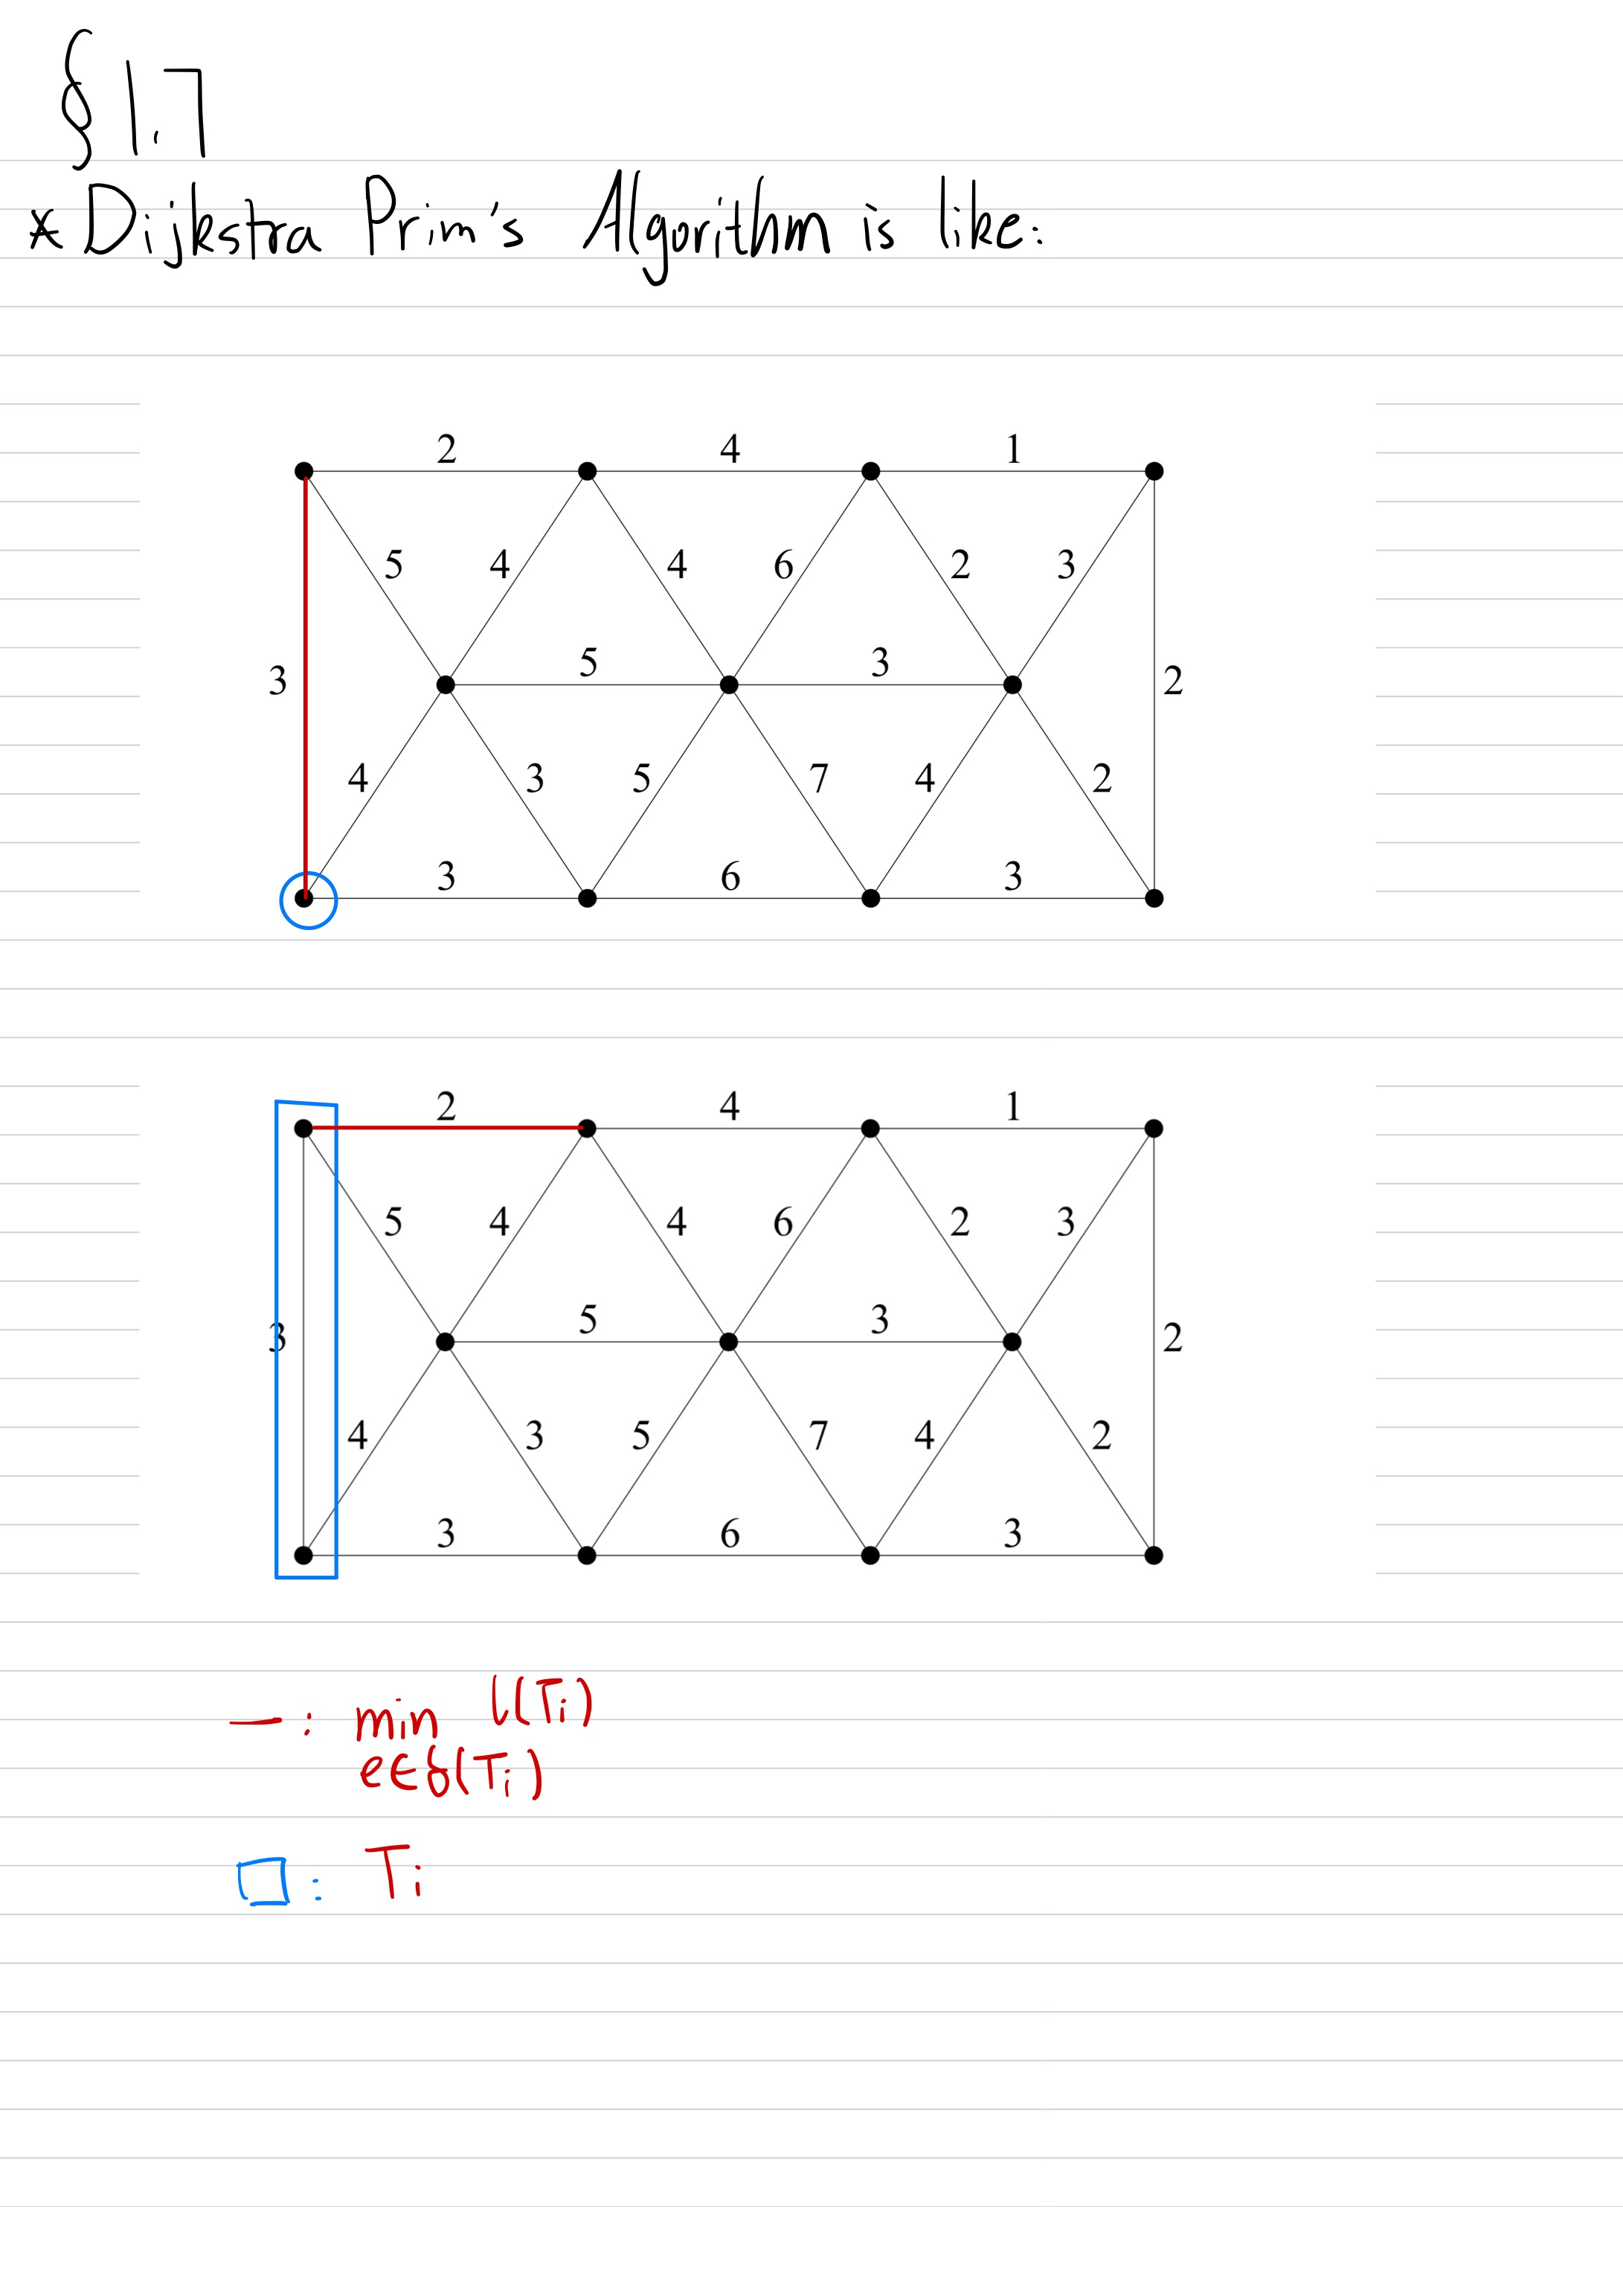
\includegraphics[width=14cm]{HW1-4.jpg}
    \end{center}
    \begin{center}
        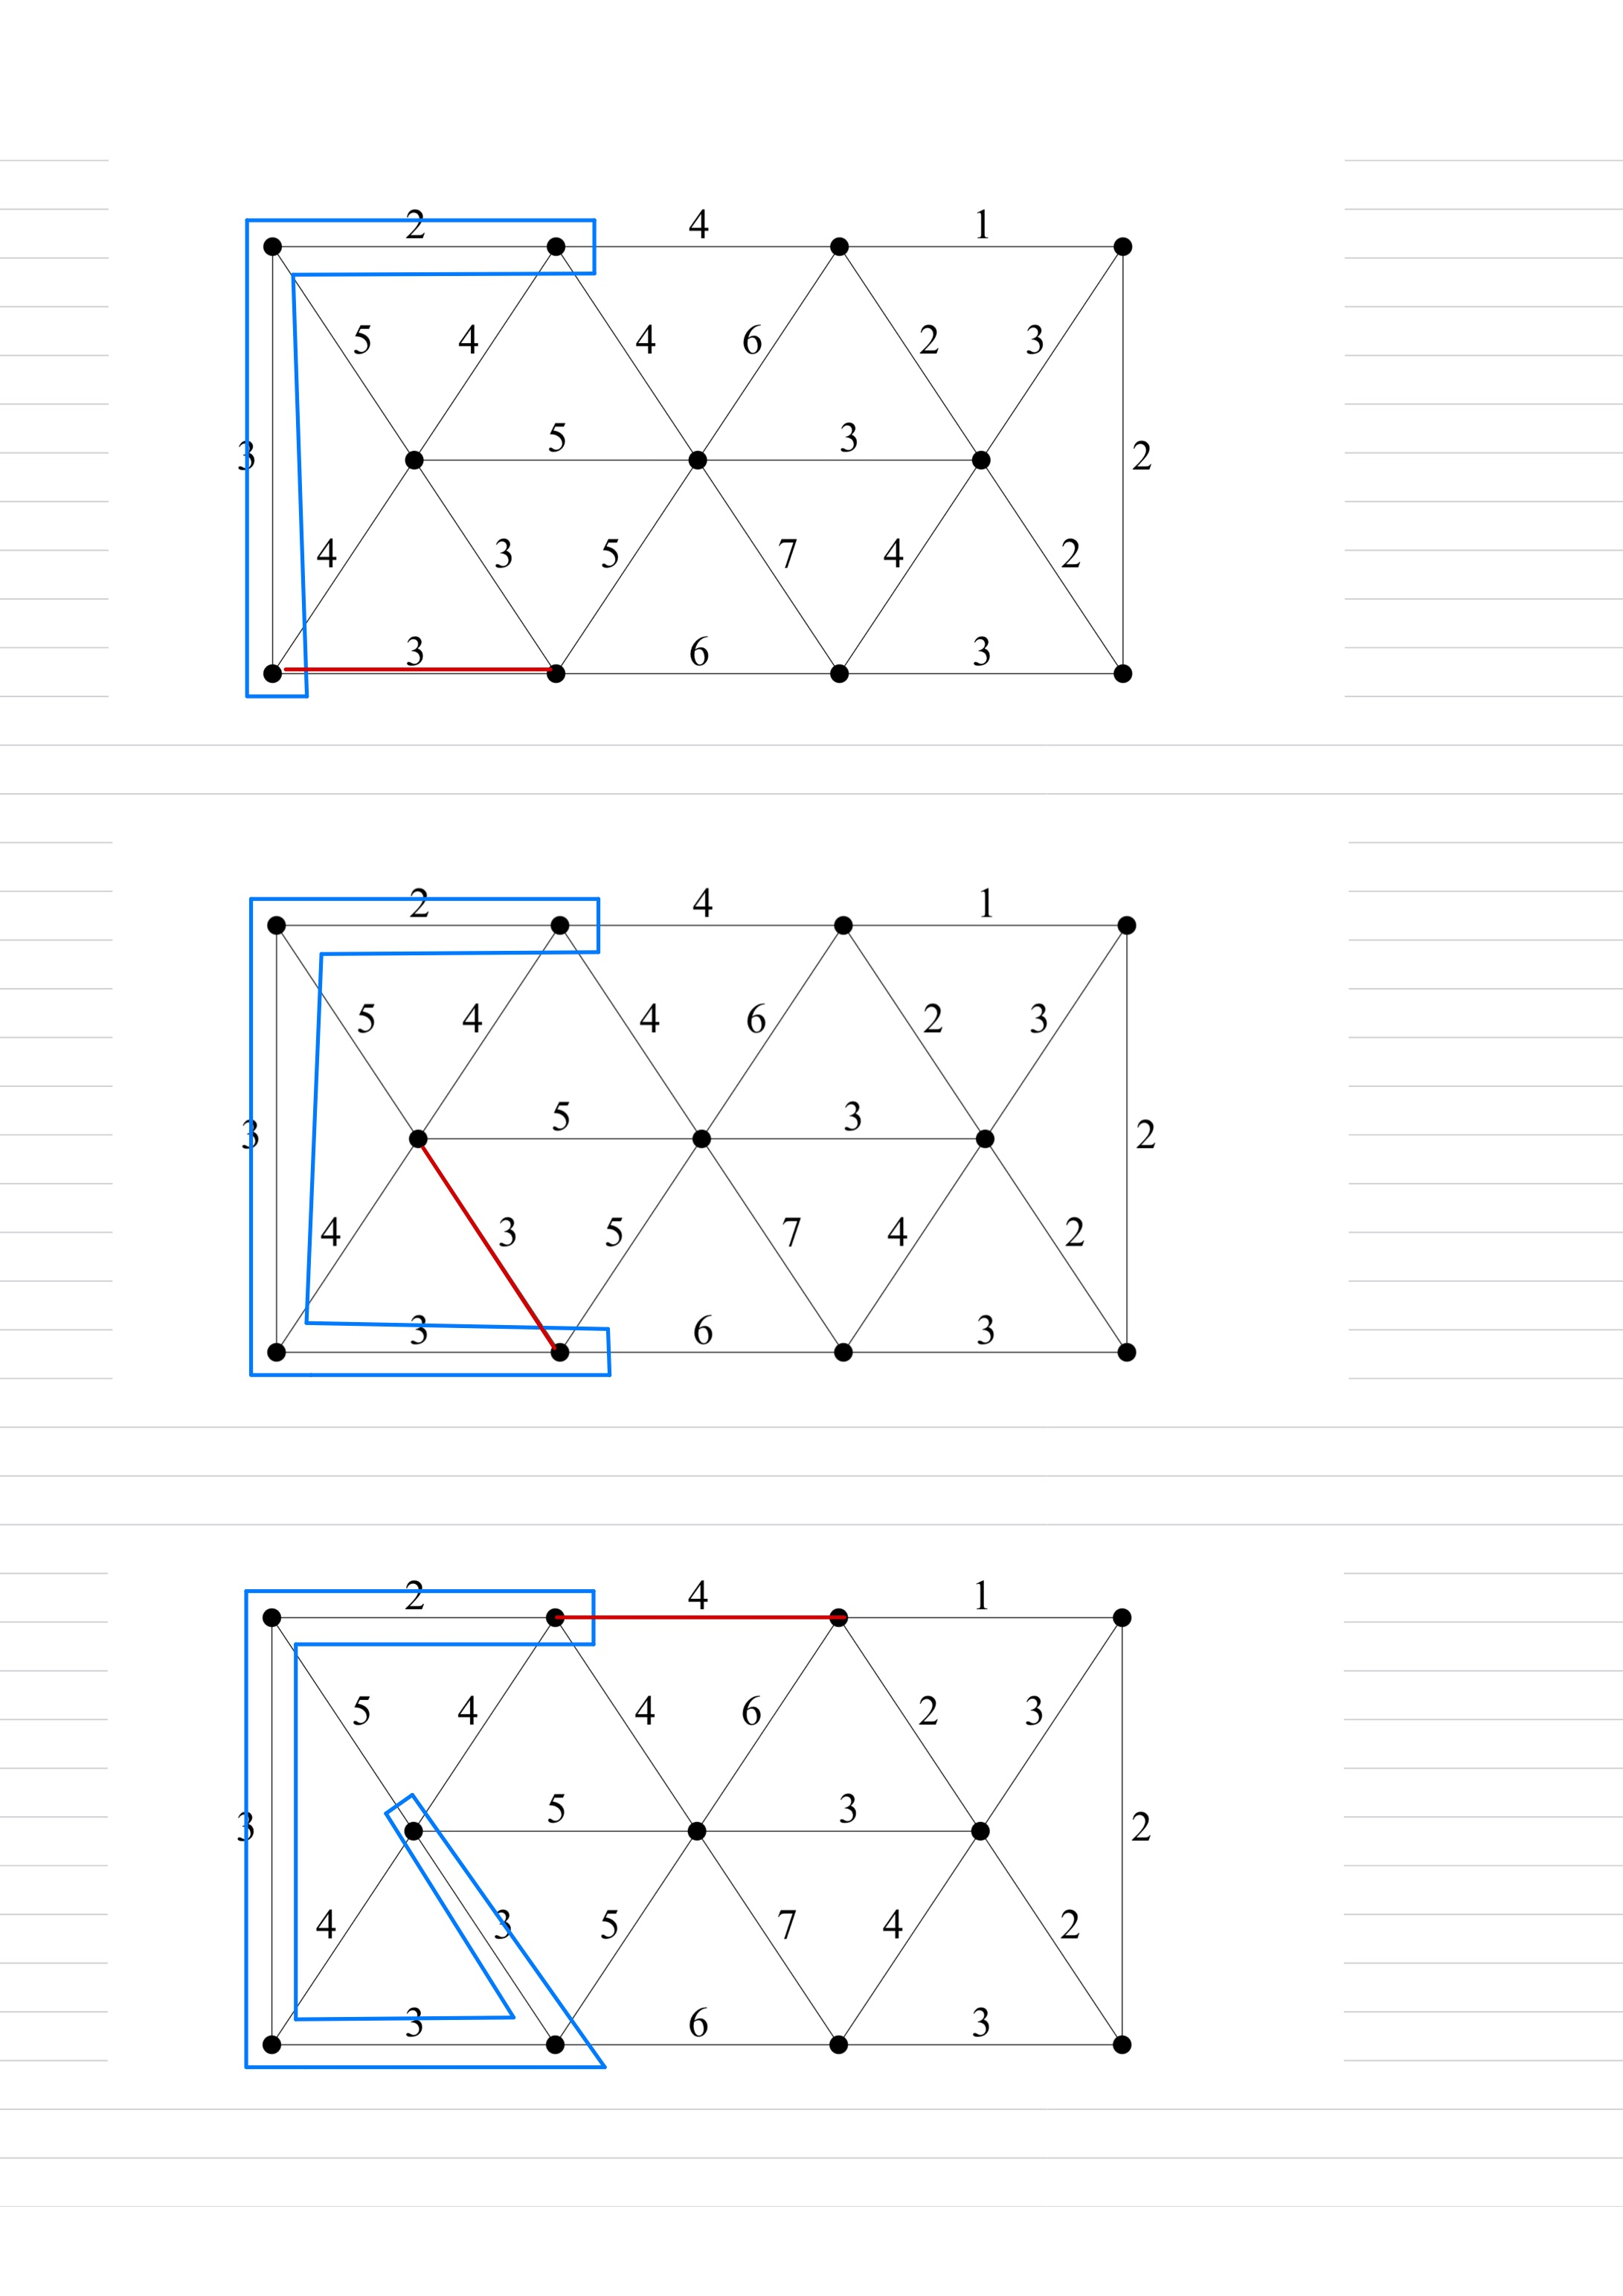
\includegraphics[width=14cm]{HW1-5.jpg}
    \end{center}
    \begin{center}
        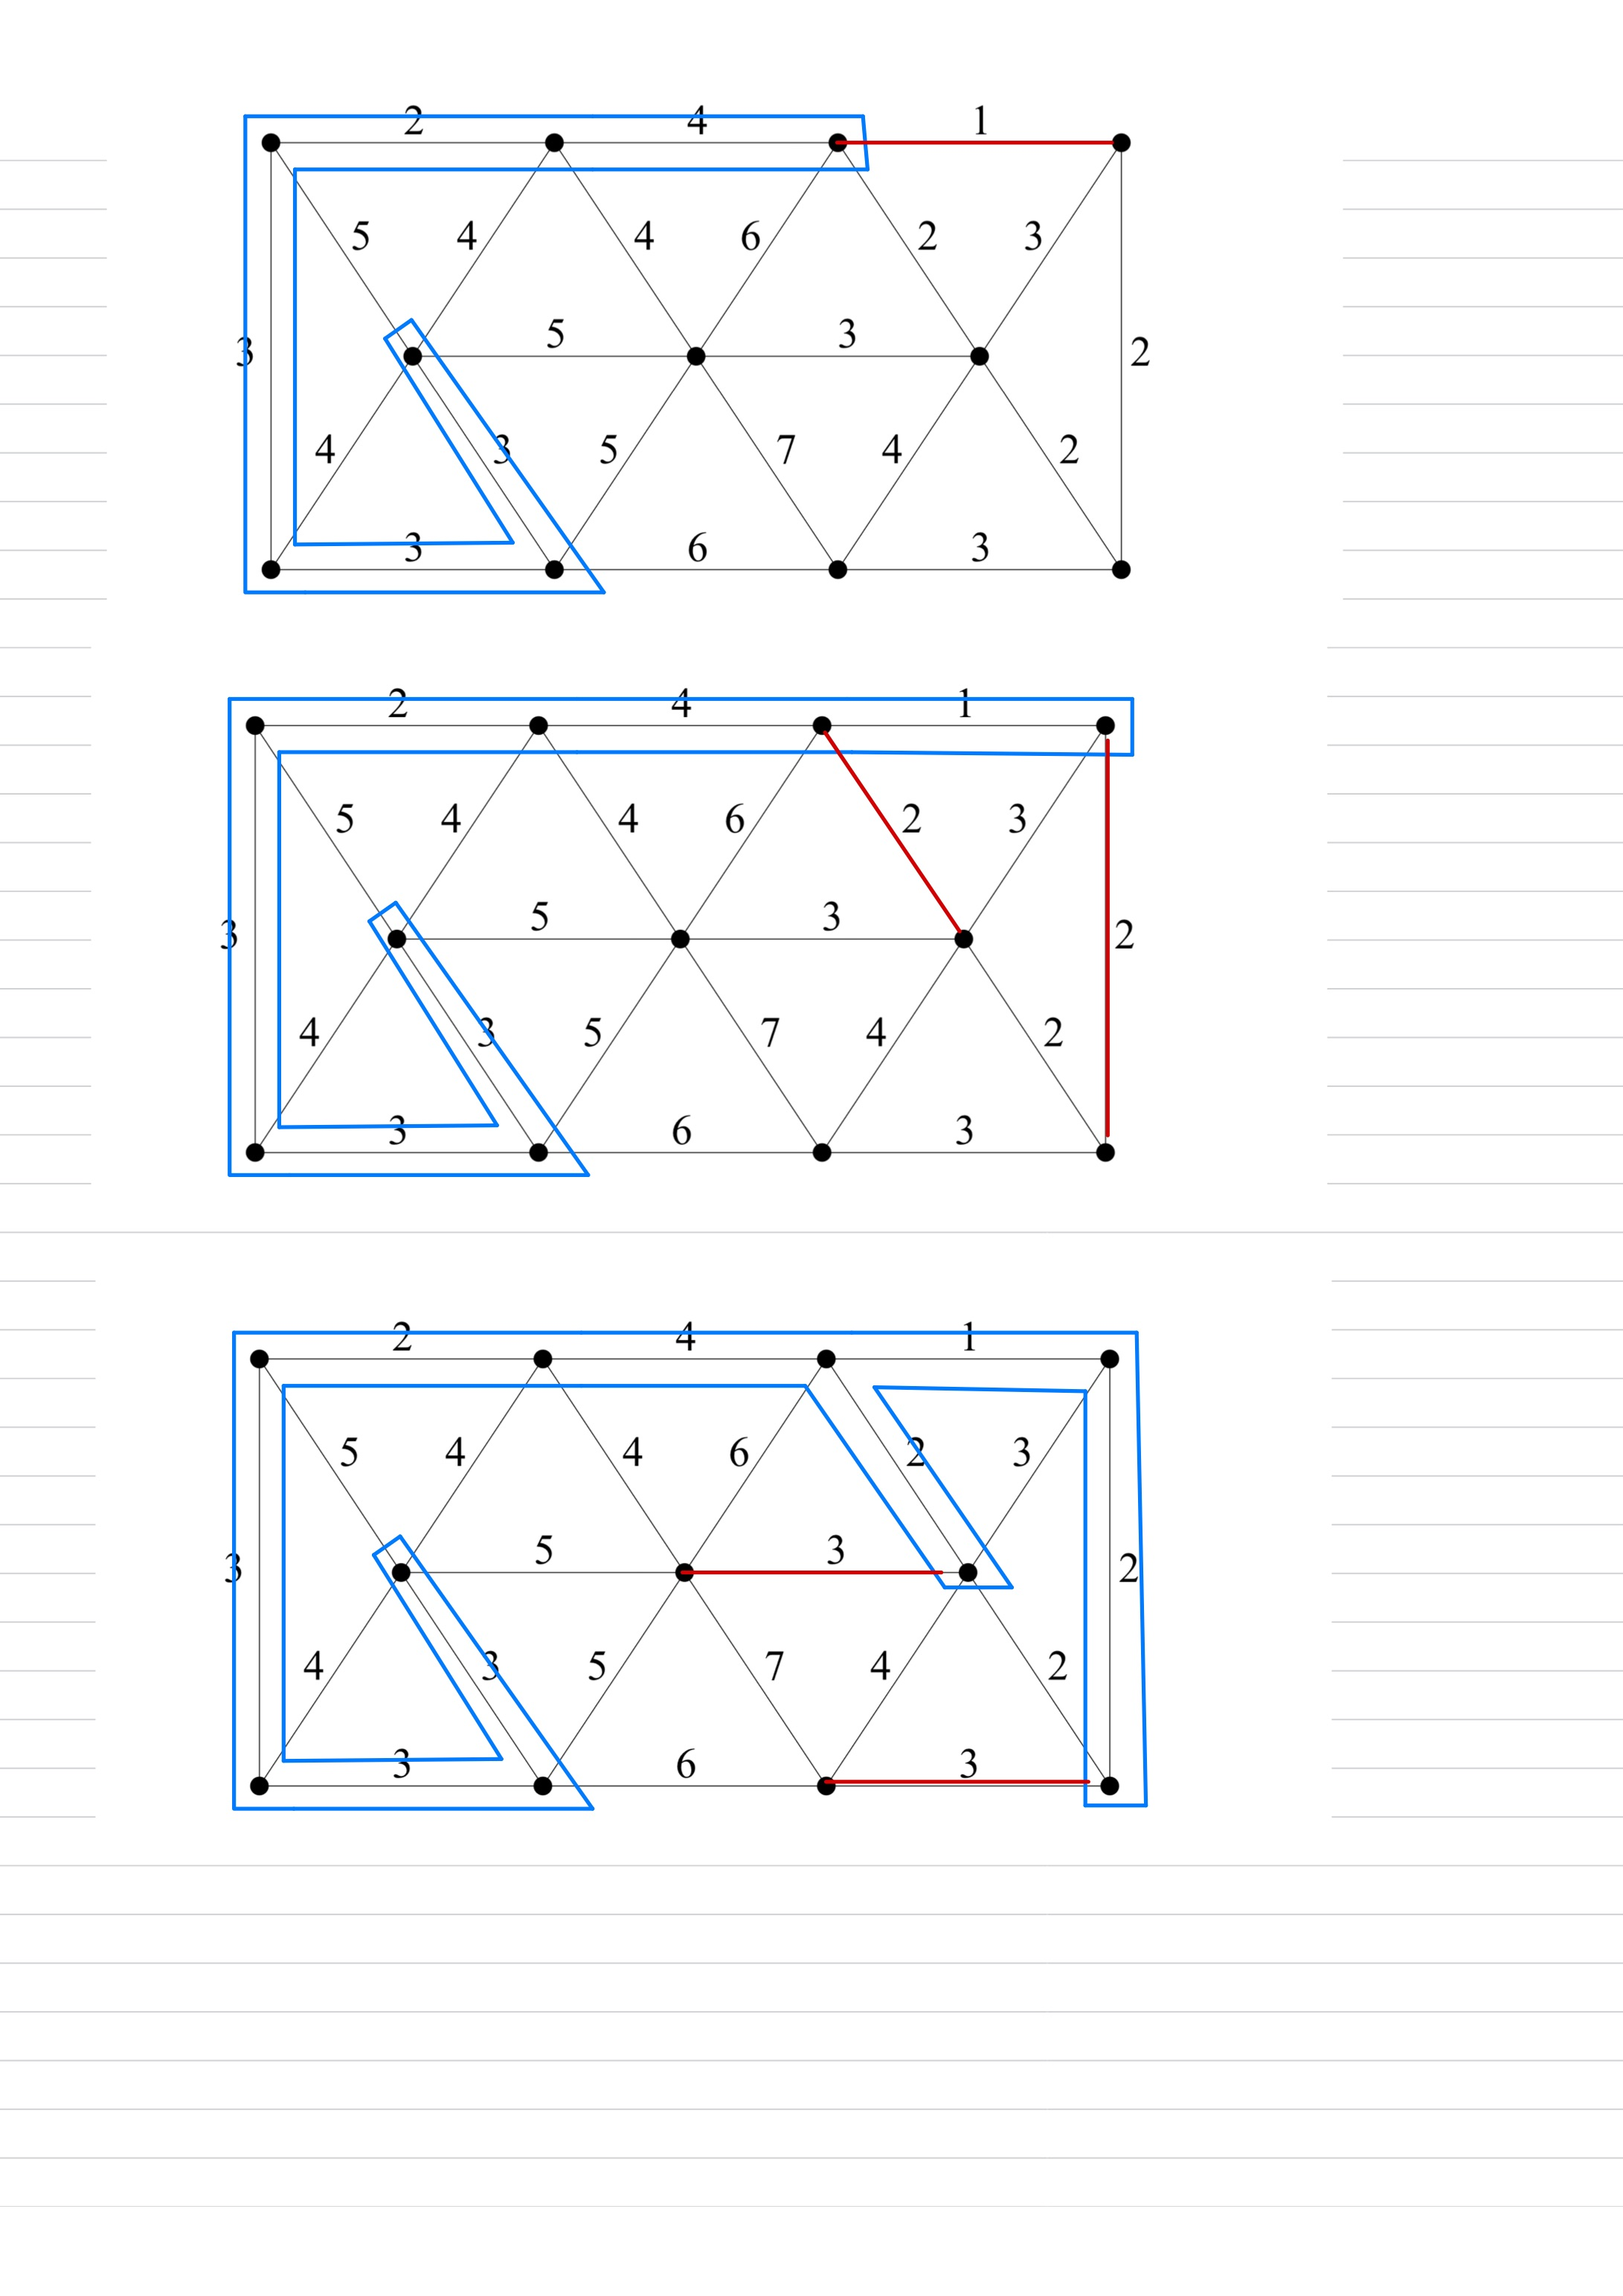
\includegraphics[width=14cm]{HW1-6.jpg}
    \end{center}
    \begin{center}
        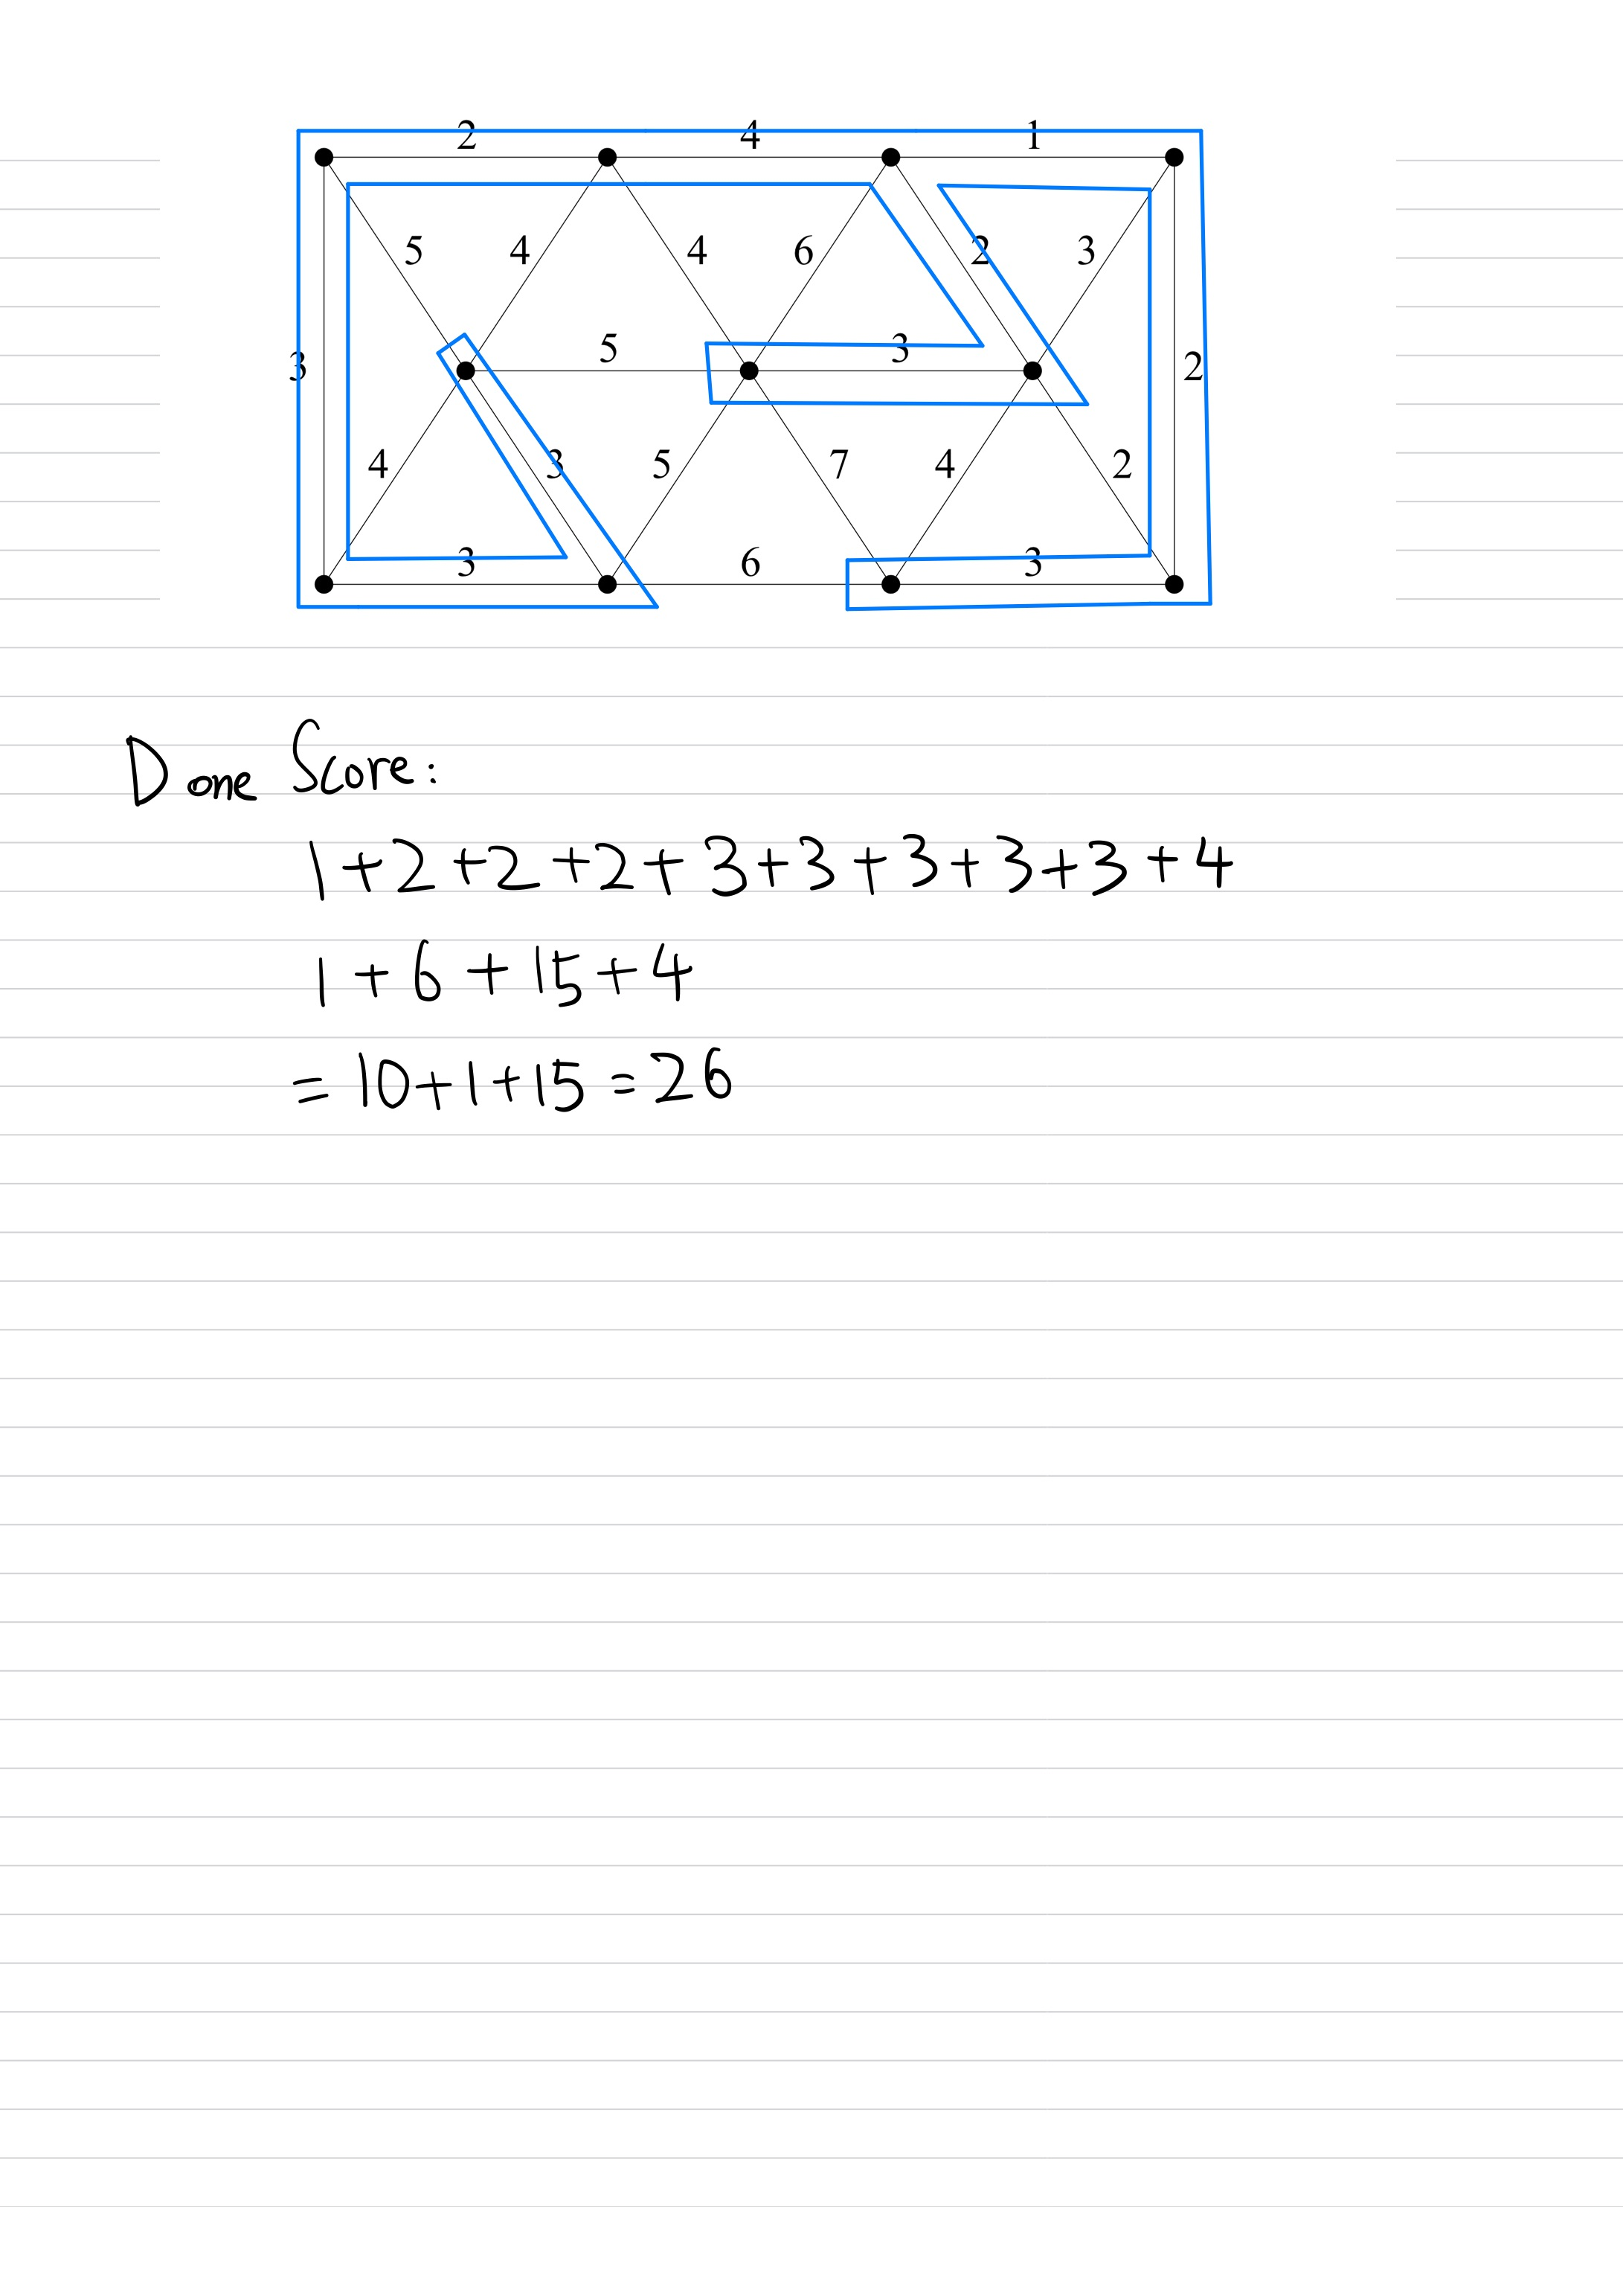
\includegraphics[width=14cm]{HW1-7.jpg}
    \end{center}
    \begin{center}
        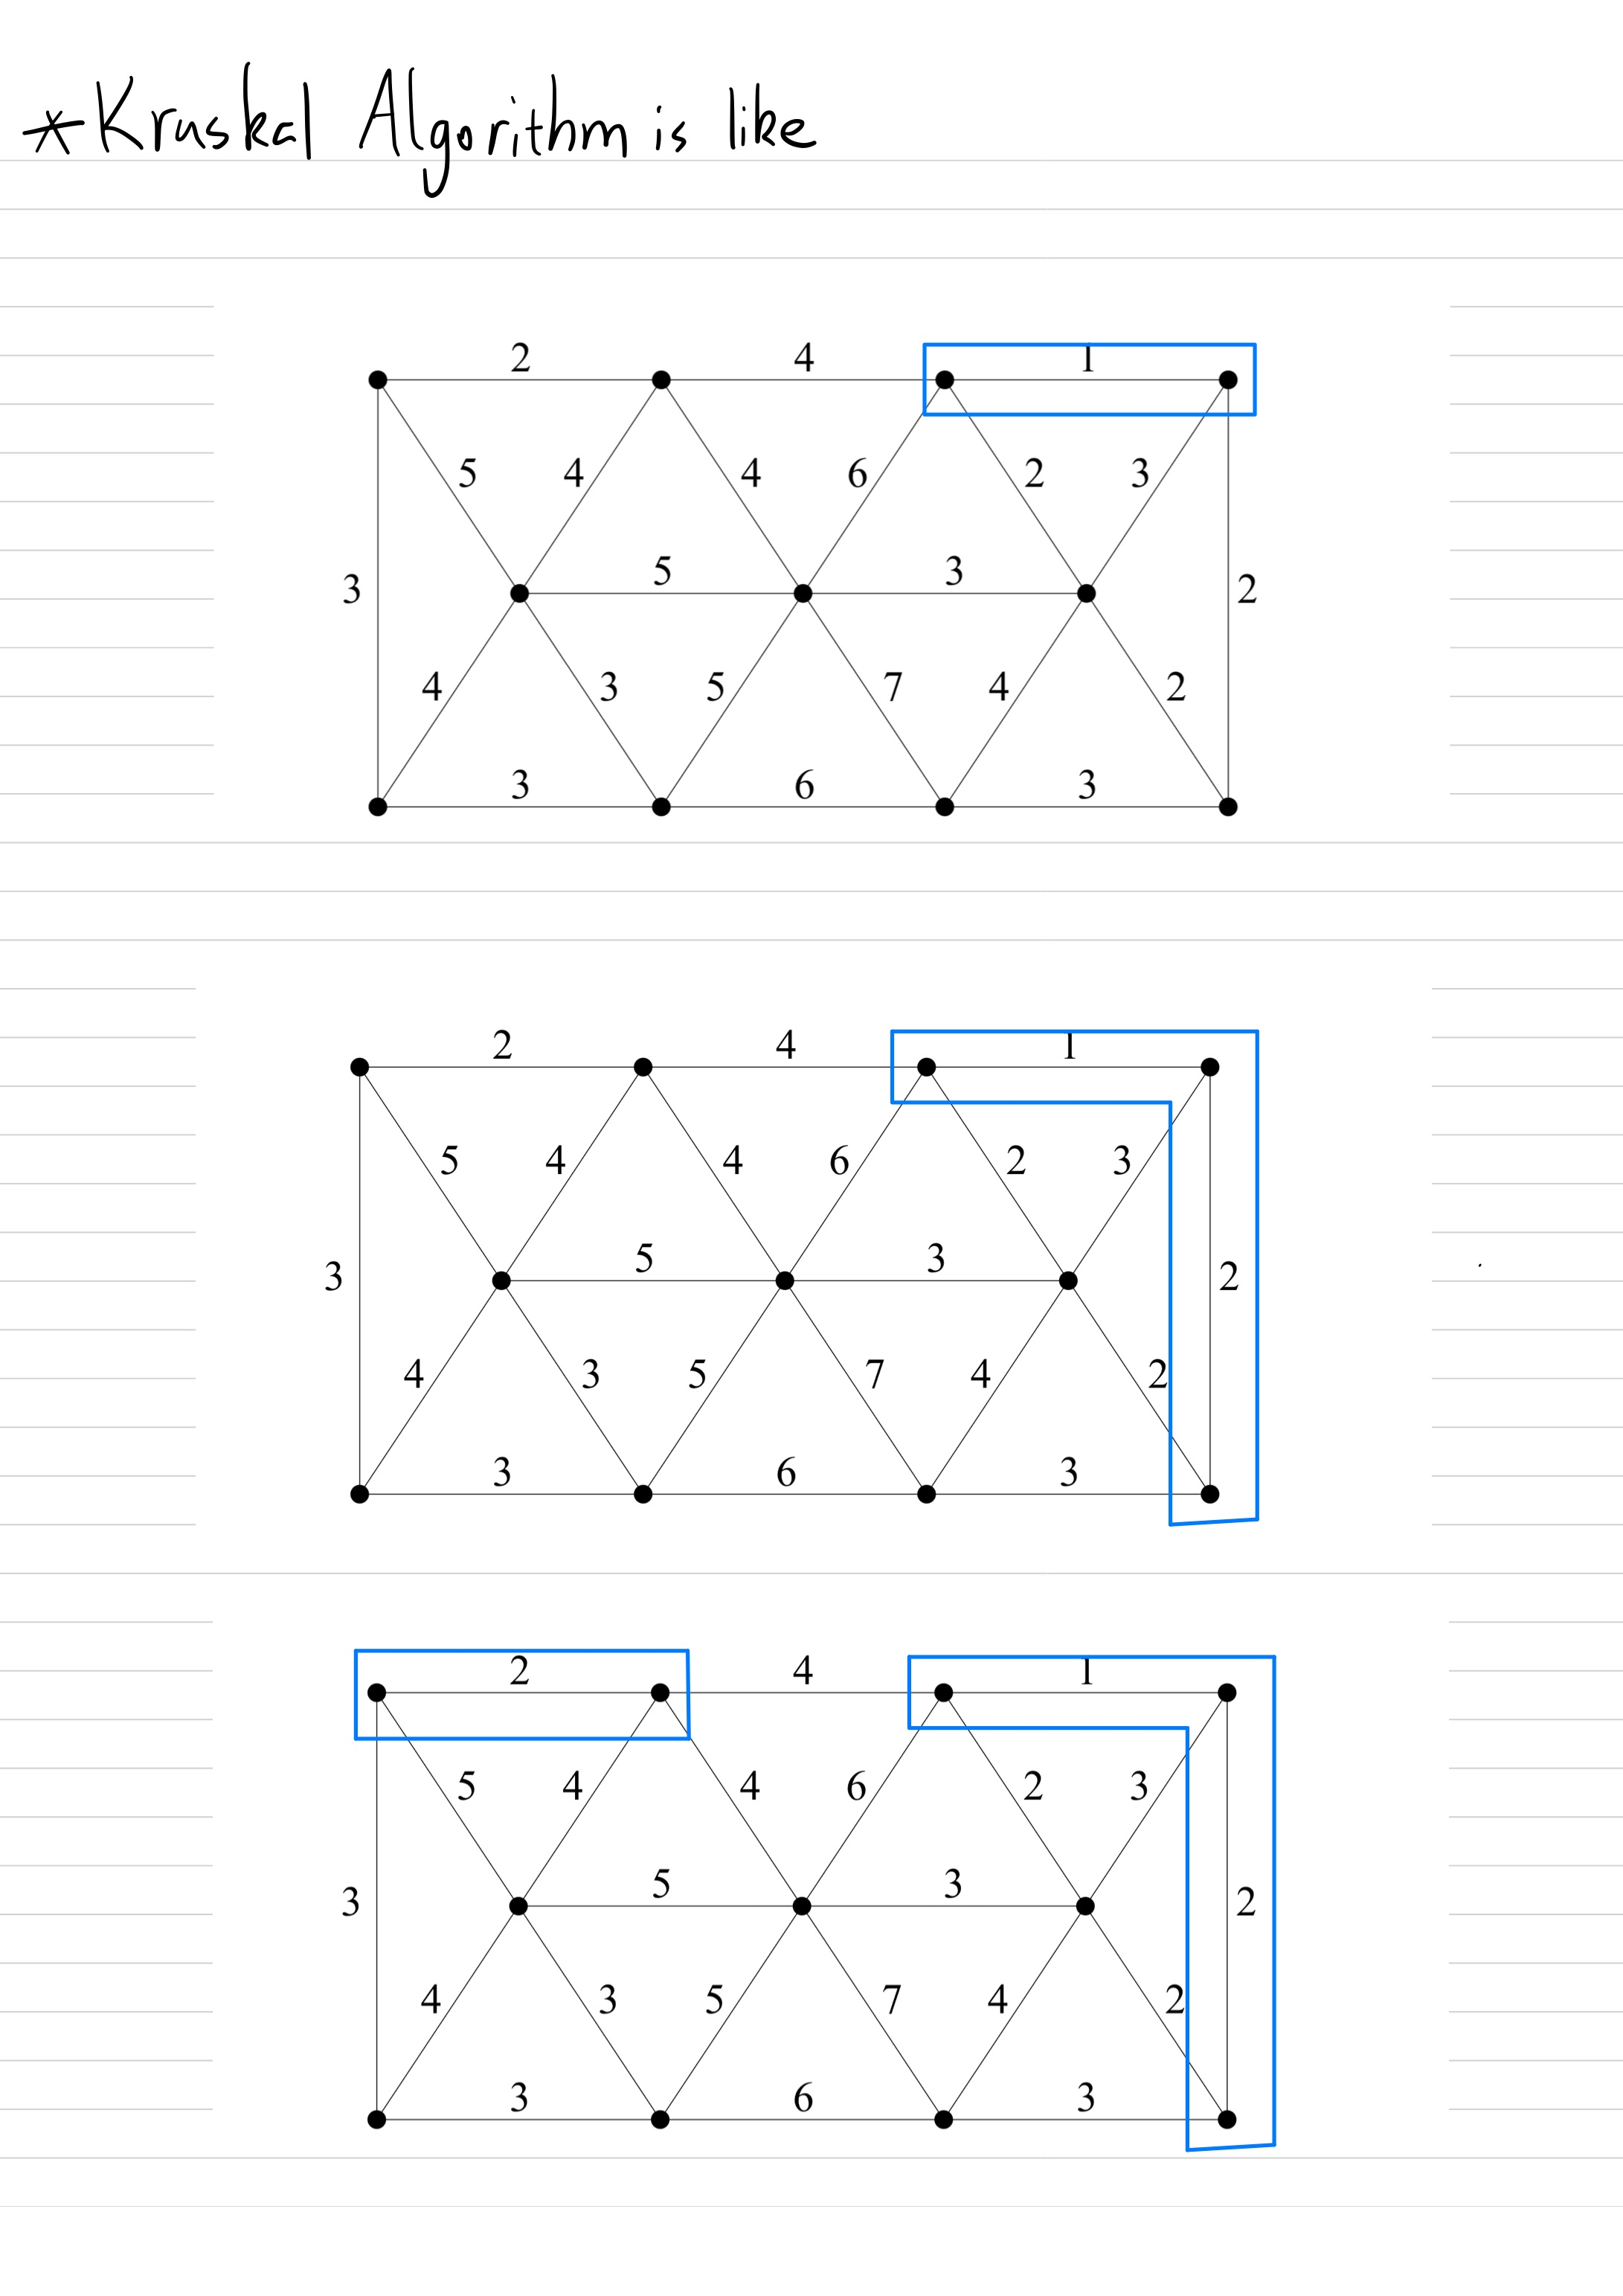
\includegraphics[width=14cm]{HW1-8.jpg}
    \end{center}
    \begin{center}
        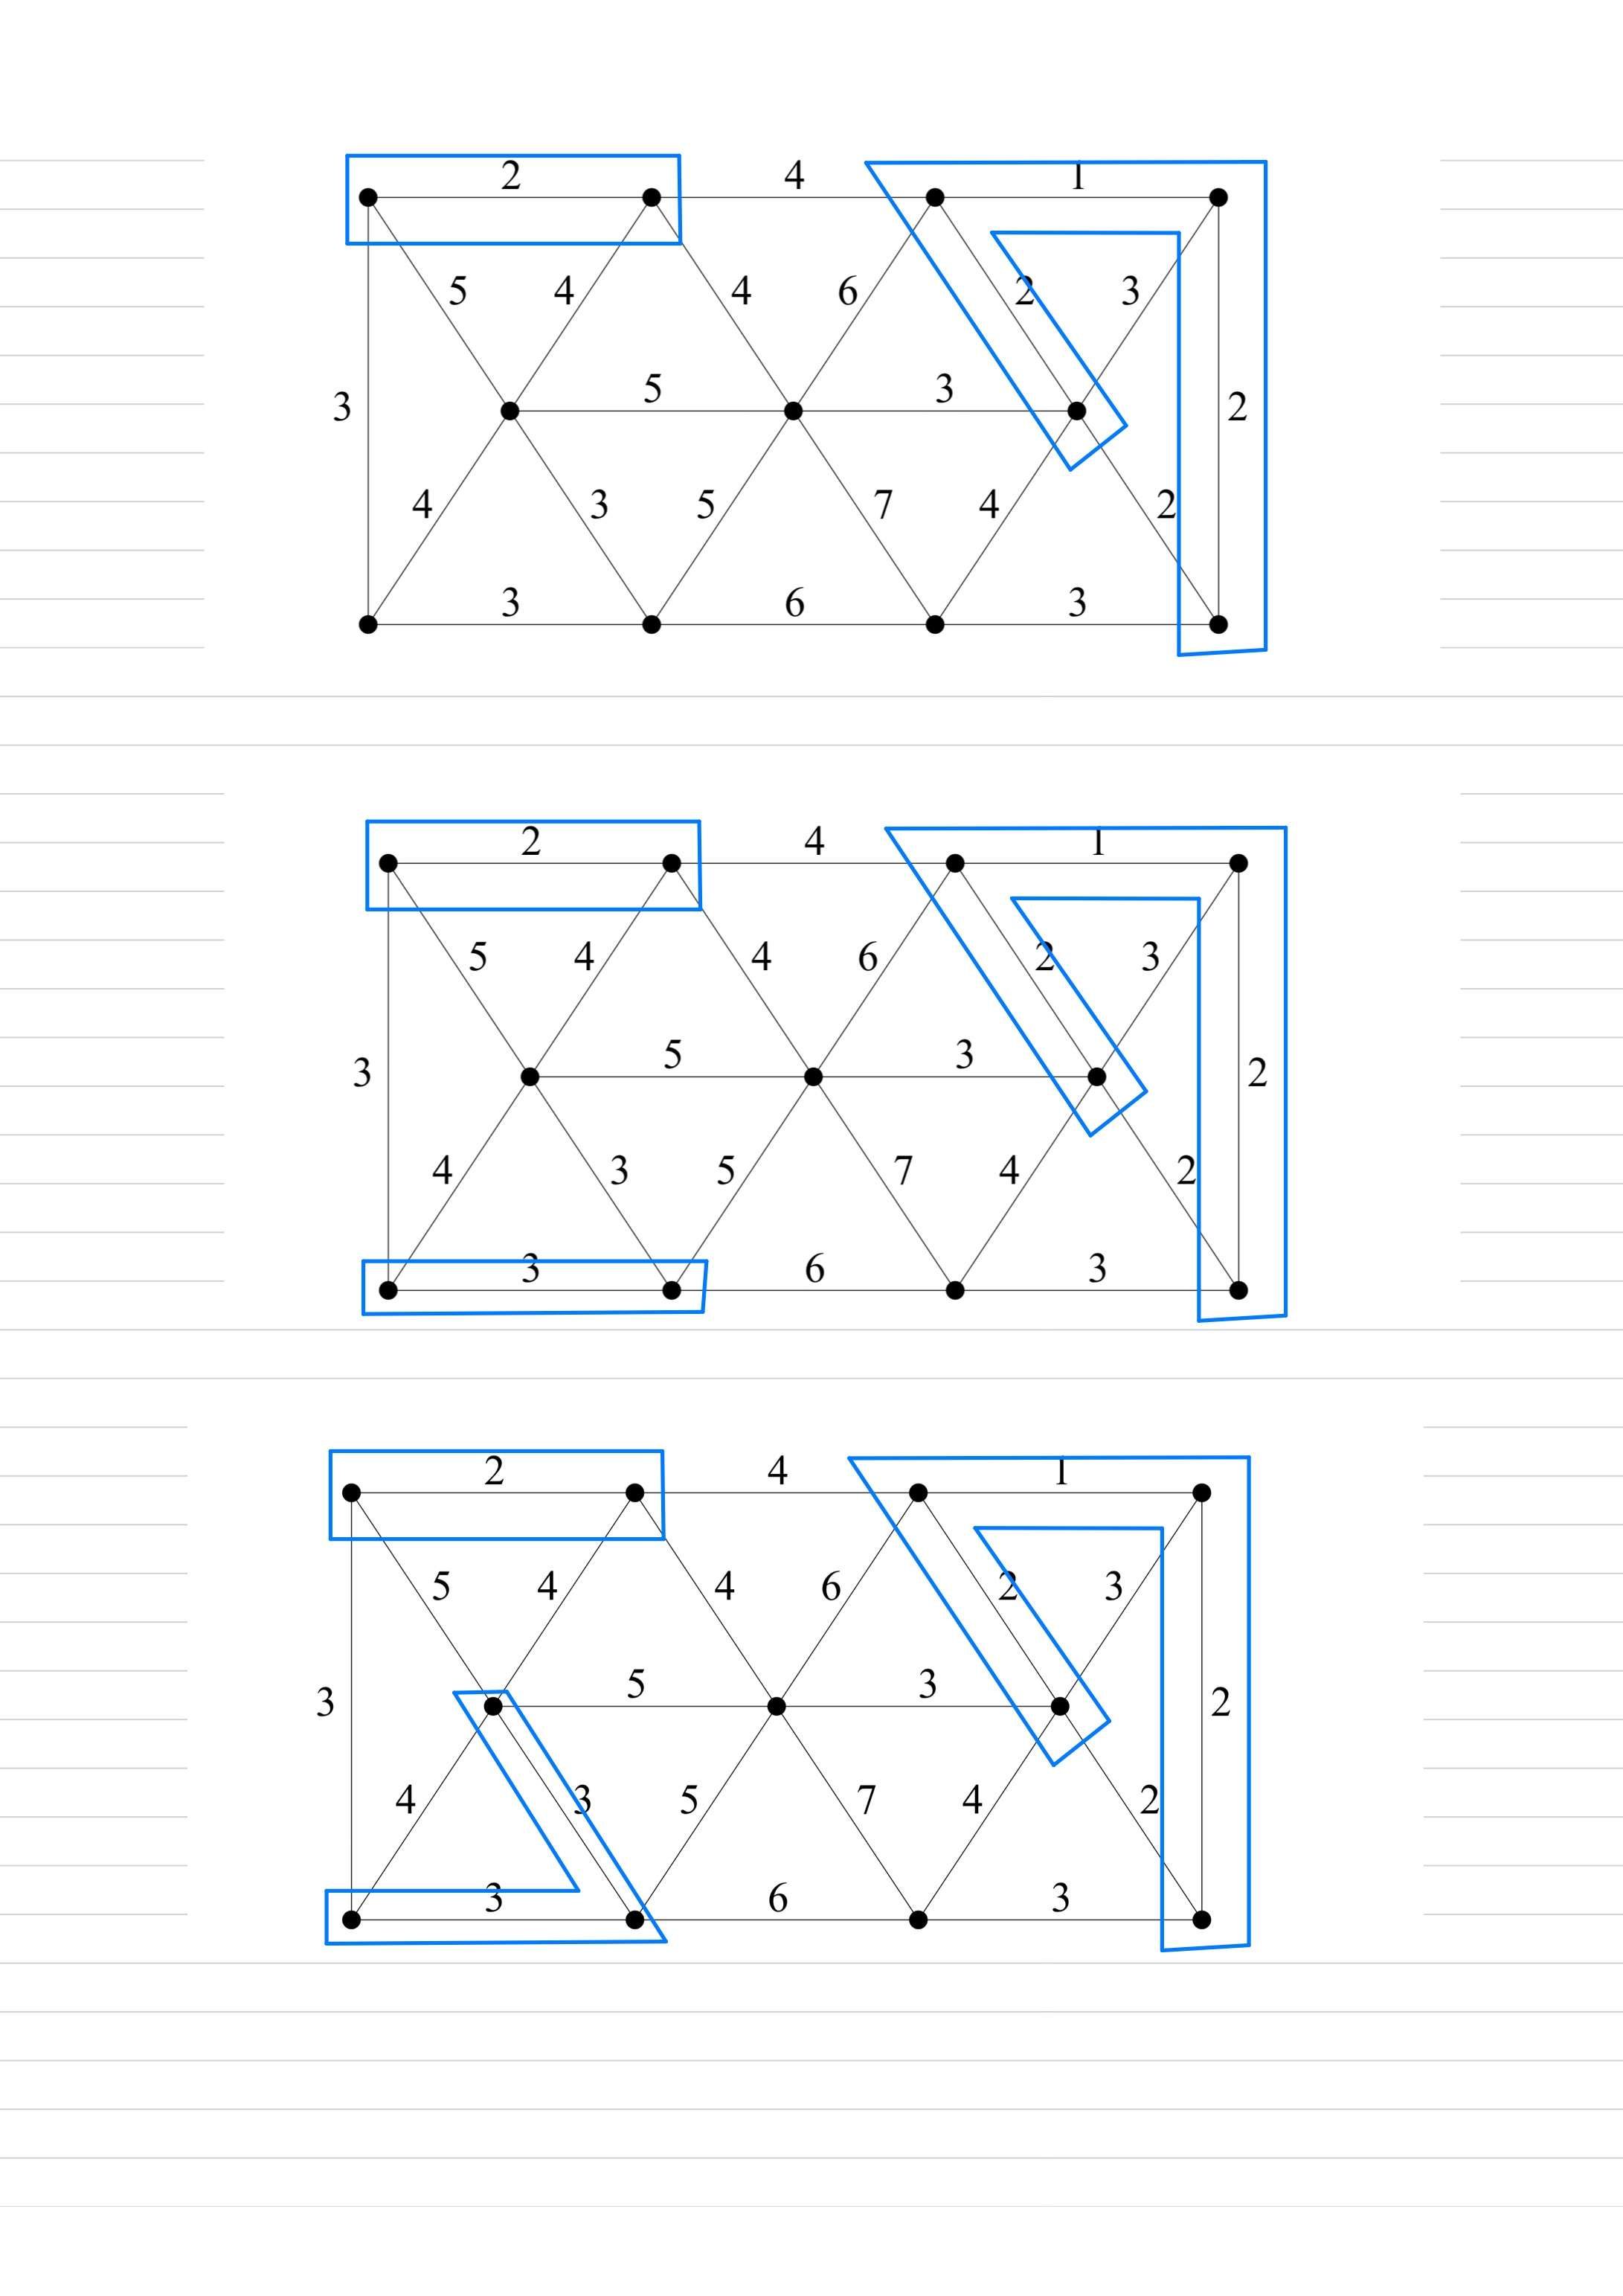
\includegraphics[width=14cm]{HW1-9.jpg}
    \end{center}
    \begin{center}
        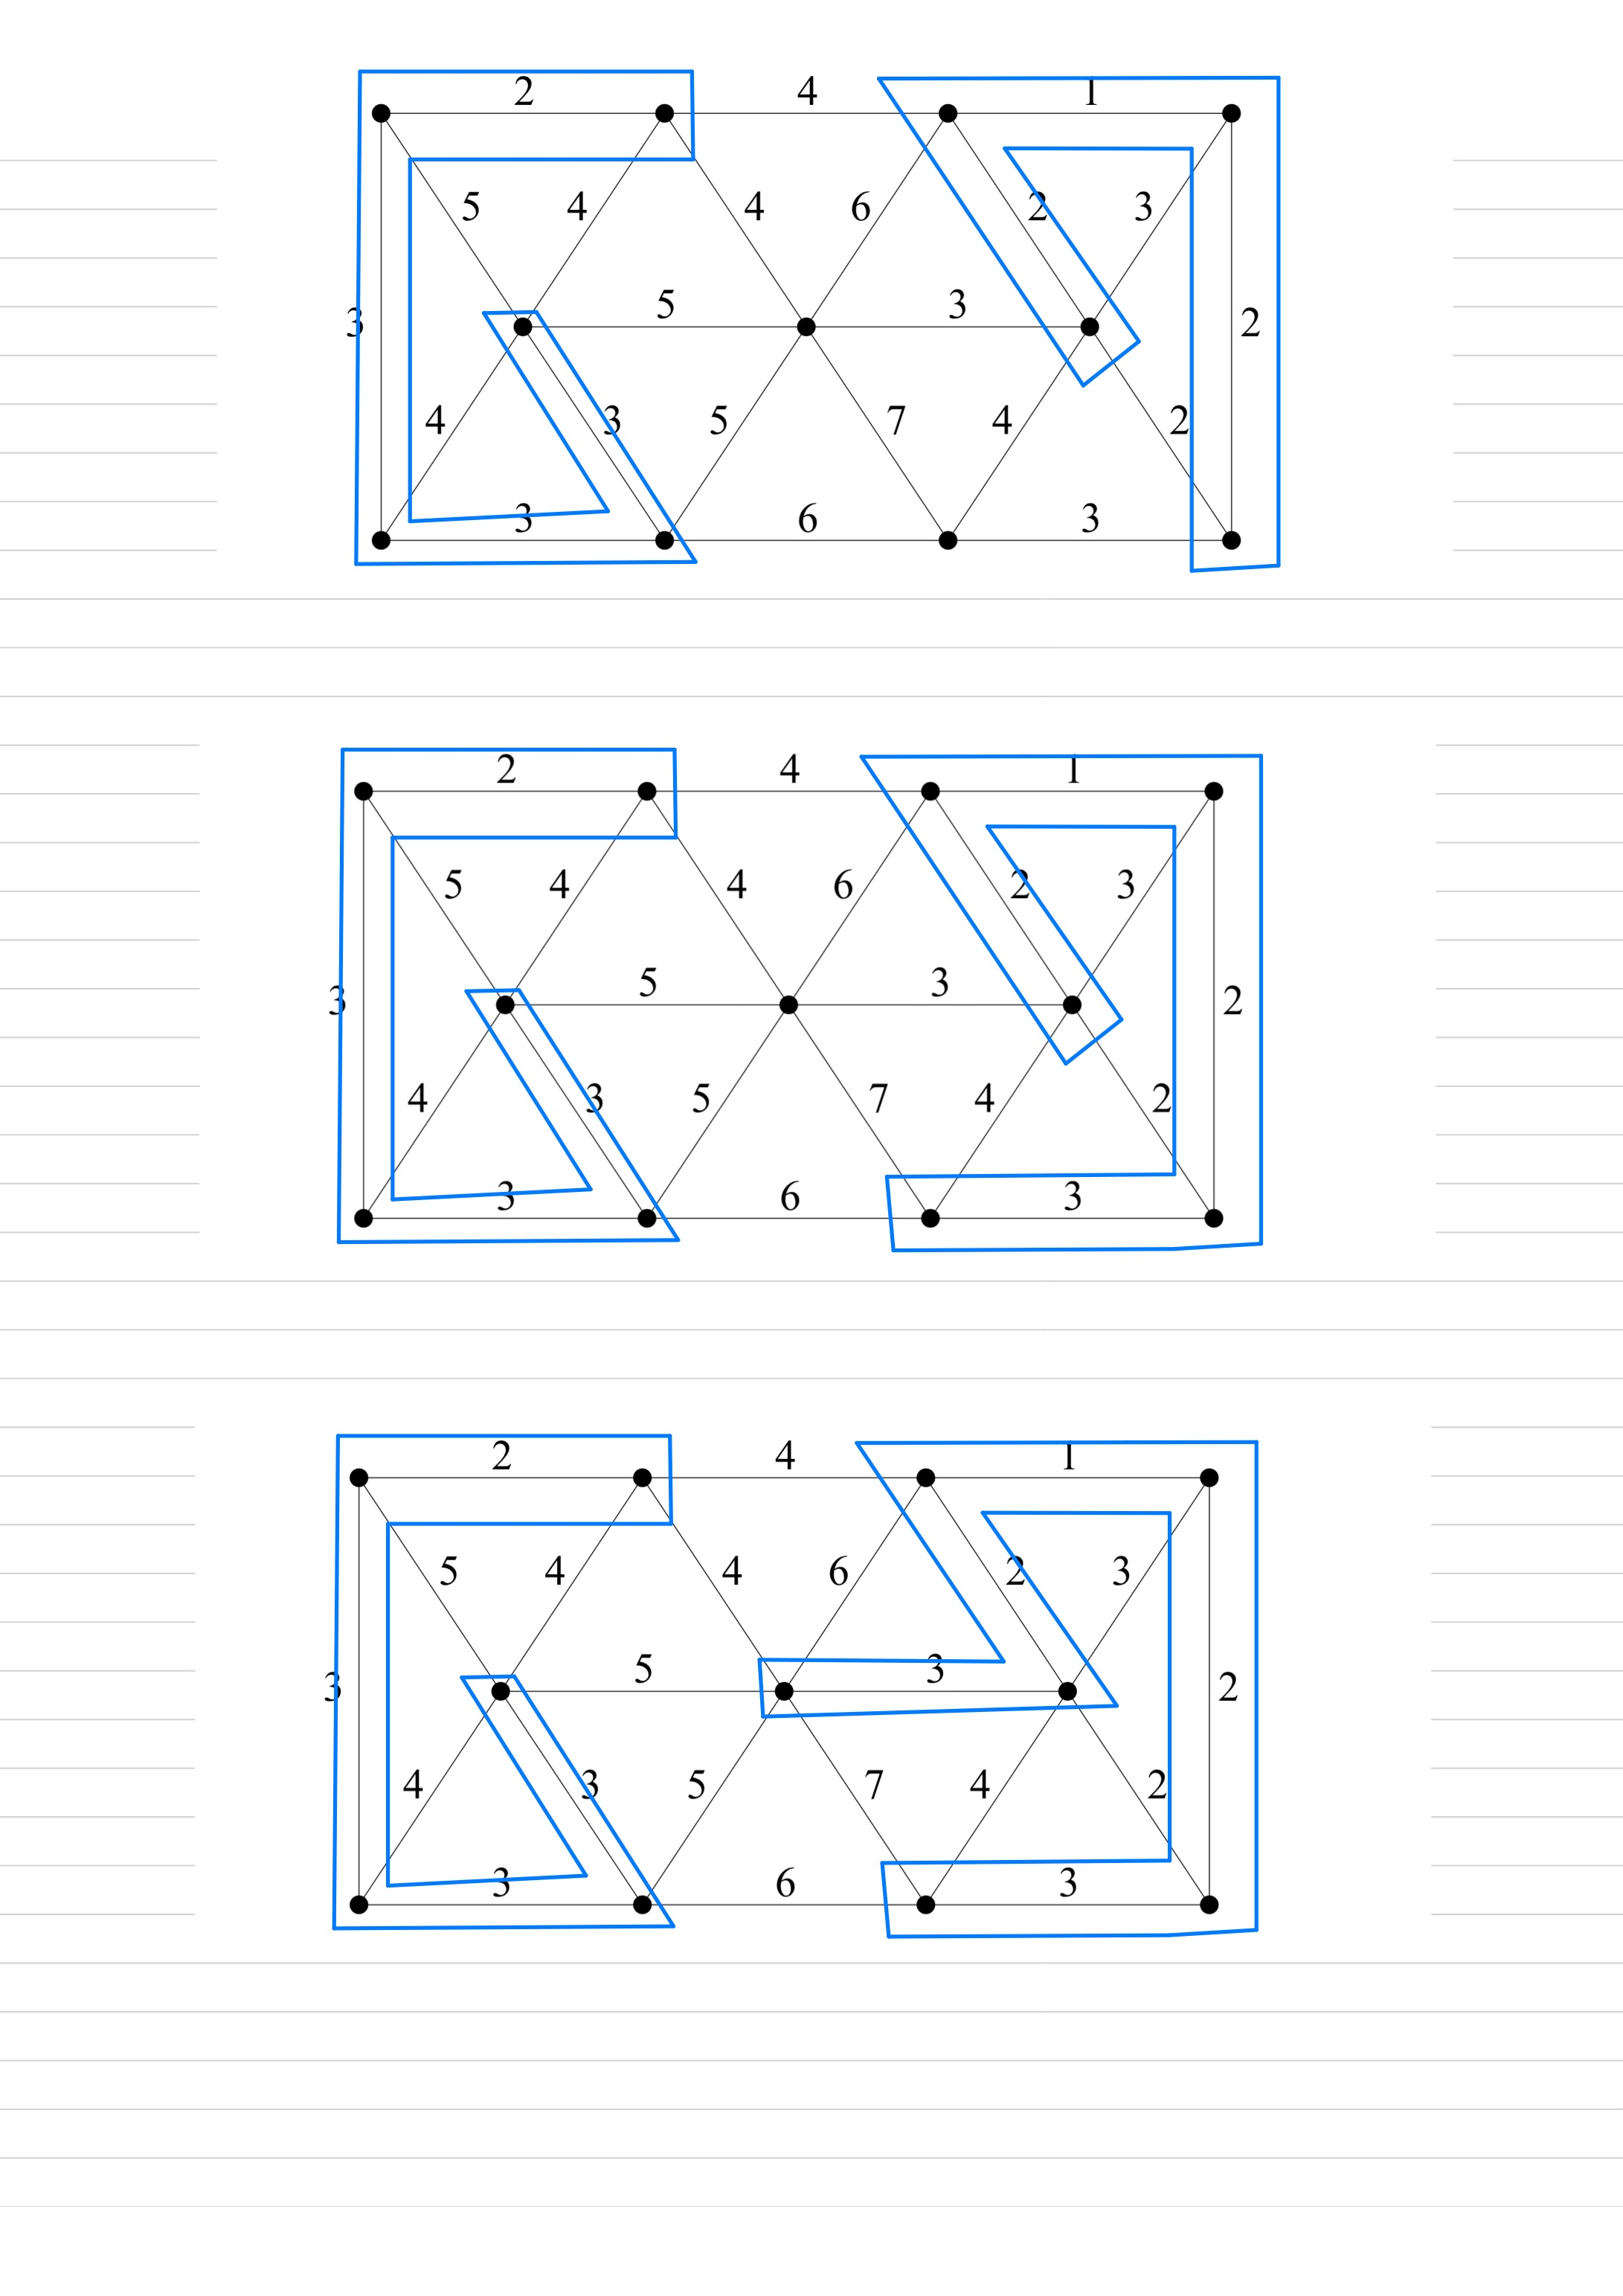
\includegraphics[width=14cm]{HW1-10.jpg}
    \end{center}
    \begin{center}
        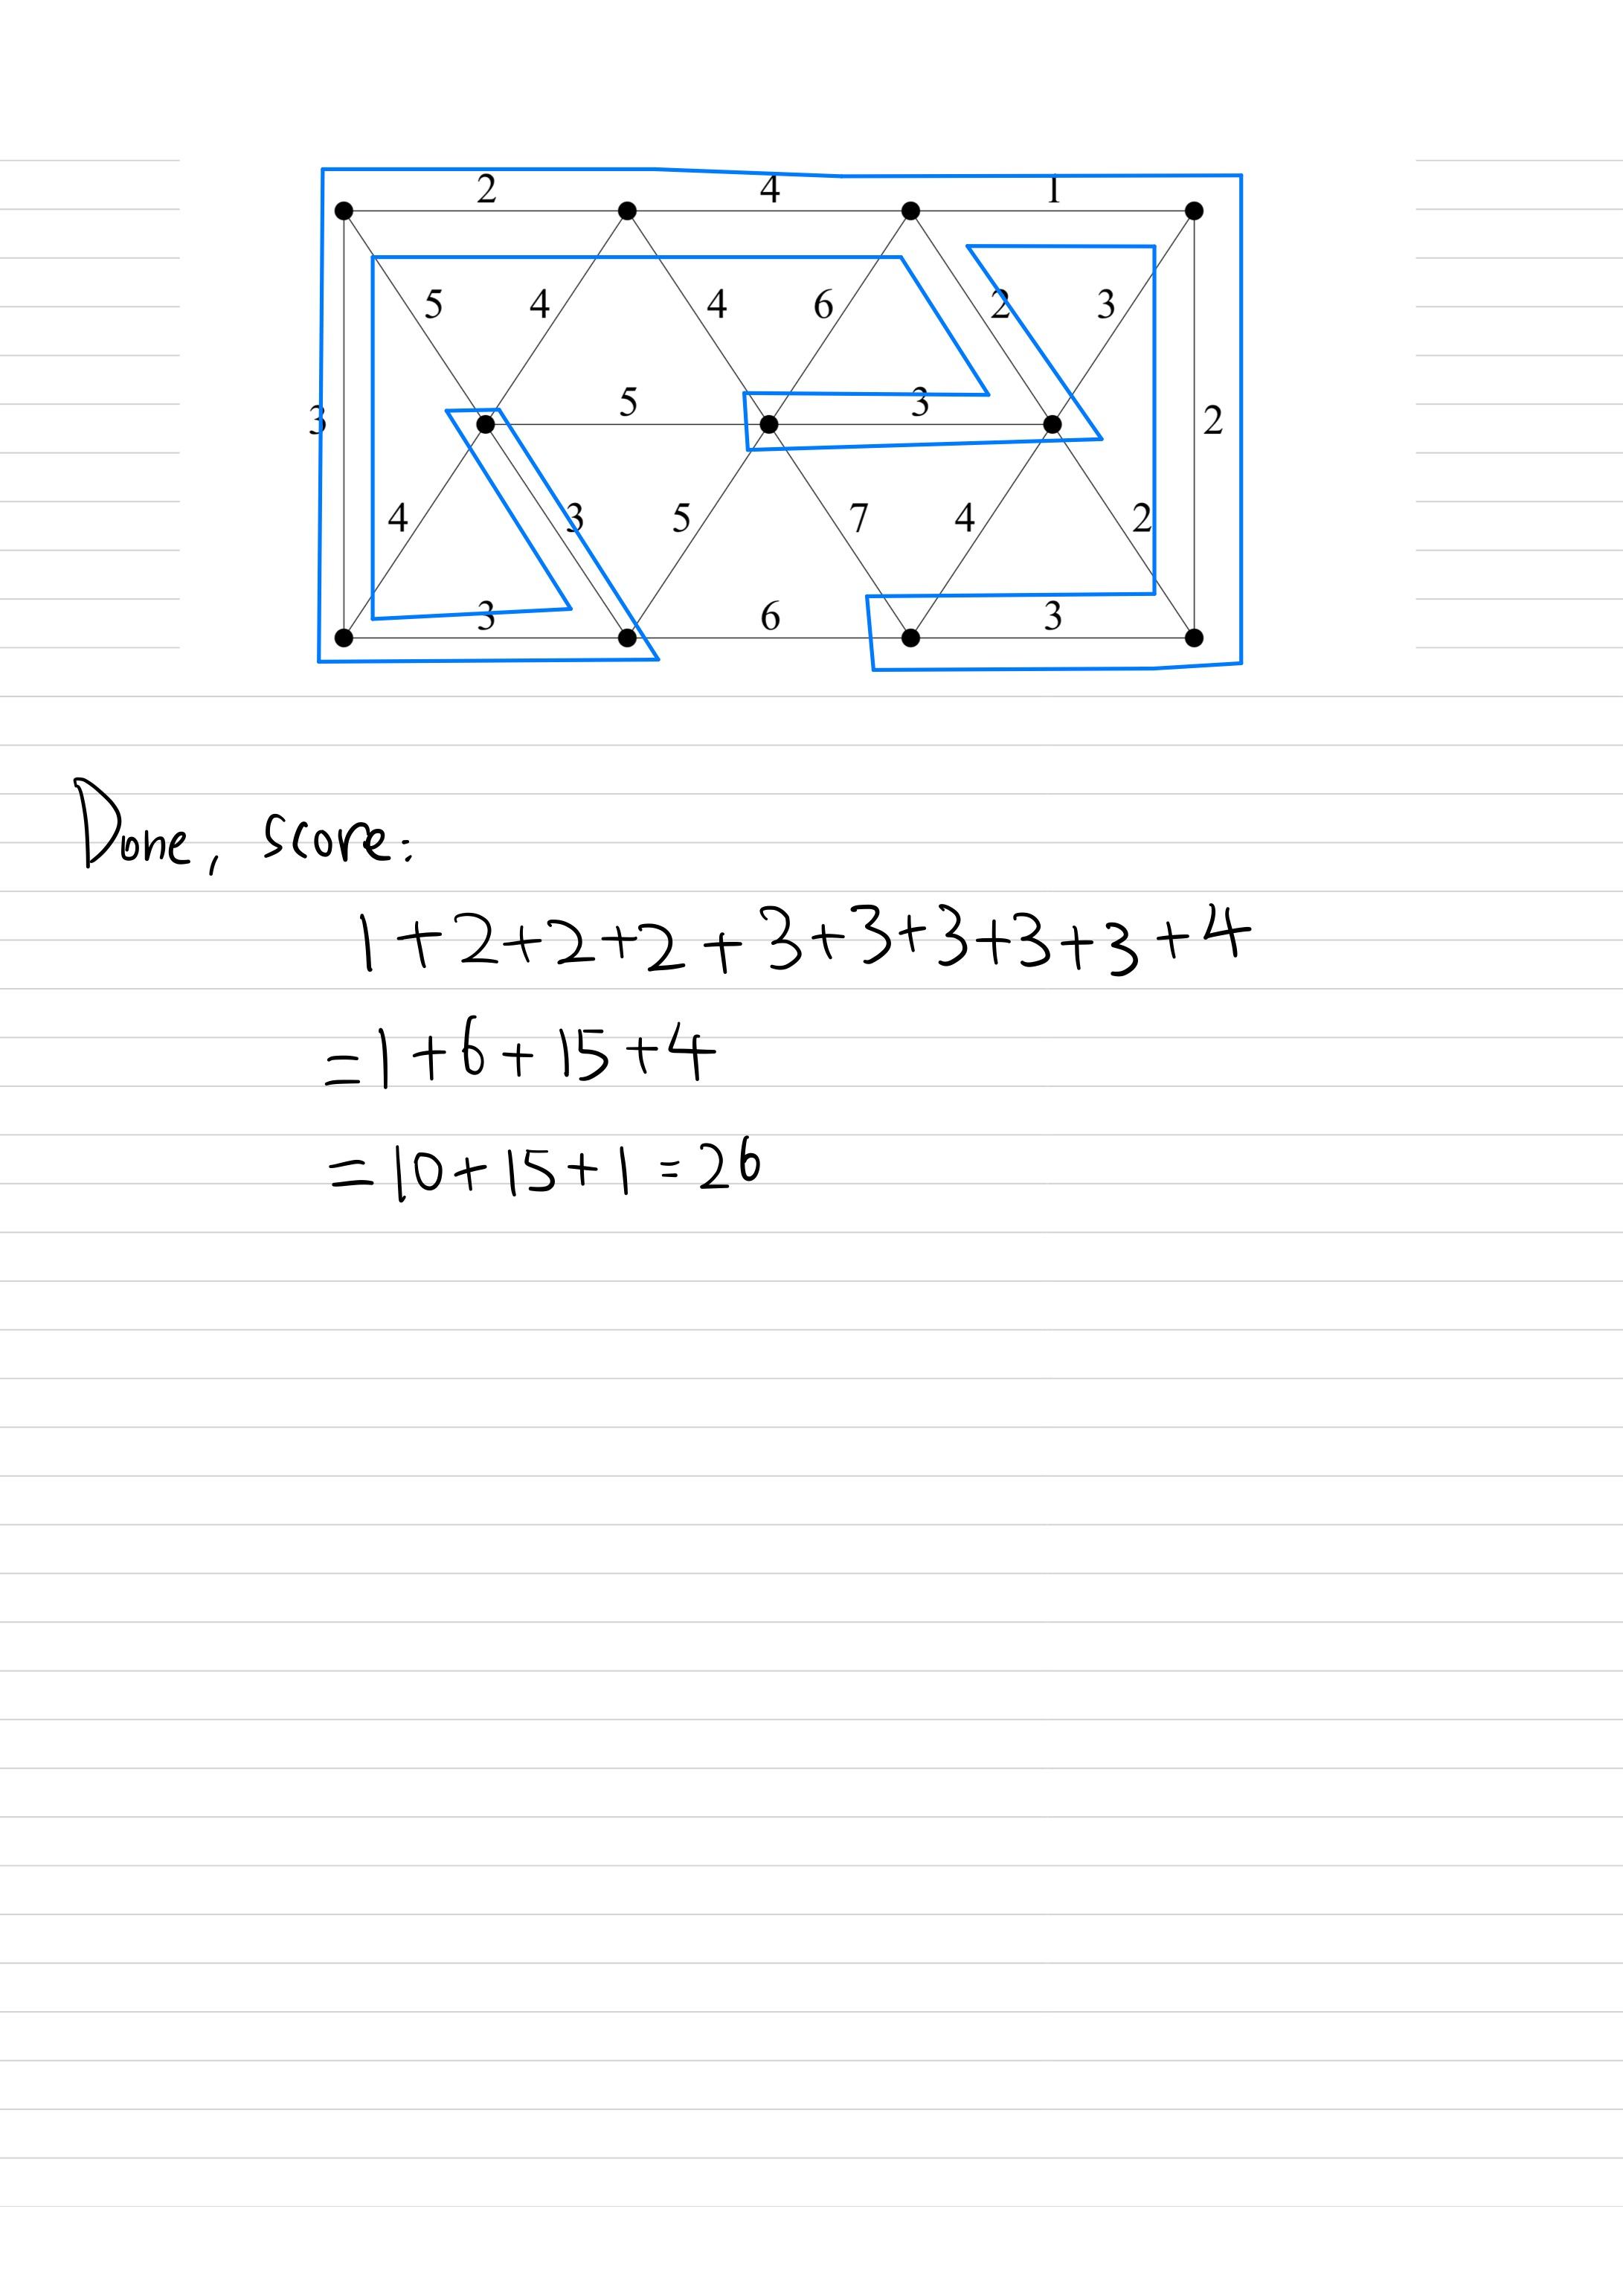
\includegraphics[width=14cm]{HW1-11.jpg}
    \end{center}
\section{1.8}
    I wrote code to do the job (I tried by hands but it took me several hours and produced the wrong results I give up) and here is my Julia Code: 
    \begin{lstlisting}
function Cities()
return ["ame", "ams","ape", "arn", "ass", "boz", "bre", "ein", "ens", 
    "s-g", "gro", "Haa", "dh", "s-h", "hil", "lee", "maa", "mid", "nij", "roe",
    "rot,", "utr", "win", "zut","zwo"
] end

function GetNameListCrossProduct()
    NameList = Cities
    n = NameList |> length
    N = fill(("", ""), n, n)
    for i = 1:n, j = 1:n
        N[i, j] = (NameList[i], NameList[j])
    end
return N end

function GetDistances()
    M = 
    [0.0 47 47 46 139 123 86 111 114 81 164 67 126 73 18 147 190 176 63 141 78 20 109 65 70;
    47 0 89 92 162 134 100 125 156 57 184 20 79 87 30 132 207 175 109 168 77 40 151 107 103;
    47 89 0 25 108 167 130 103 71 128 133 109 154 88 65 129 176 222 42 127 125 67 66 22 41;
    46 92 25 0 132 145 108 78 85 116 157 112 171 63 64 154 151 200 17 102 113 59 64 31 66;
    139 162 108 132 0 262 225 210 110 214 25 182 149 195 156 68 283 315 149 234 217 159 143 108 69;
    123 134 167 145 262 0 37 94 230 83 287 124 197 82 119 265 183 59 128 144 57 103 209 176 193;
    86 100 130 108 225 37 0 57 193 75 250 111 179 45 82 228 147 96 91 107 49 66 172 139 156;
    111 125 103 78 210 94 57 0 163 127 235 141 204 38 107 232 100 153 61 50 101 91 142 109 144;
    114 156 71 85 110 230 193 163 0 195 135 176 215 148 132 155 236 285 102 187 192 134 40 54 71;
    81 57 128 116 214 83 75 127 195 0 236 41 114 104 72 182 162 124 133 177 26 61 180 146 151;
    164 184 133 157 25 287 250 235 135 236 0 199 147 220 178 58 308 340 174 259 242 184 168 133 94;
    67 20 109 112 182 124 111 141 176 41 199 0 73 103 49 141 203 165 129 184 67 56 171 127 123;
    126 79 154 171 149 197 179 204 215 114 147 73 0 166 109 89 276 238 188 247 140 119 220 176 144;
    73 87 88 63 195 82 45 38 148 104 220 103 166 0 69 215 123 141 46 81 79 53 127 94 129;
    18 30 65 64 156 119 82 107 132 72 178 49 109 69 0 146 192 172 81 150 74 16 127 83 88;
    147 132 129 154 68 265 228 232 155 182 58 141 89 215 146 0 306 306 171 256 208 162 183 139 91;
    190 207 176 151 283 183 147 100 236 162 308 203 276 123 192 305 0 242 135 50 188 176 213 182 217;
    176 175 222 200 315 59 96 153 285 124 340 165 238 141 172 306 242 0 187 203 98 156 264 231 246;
    63 109 42 17 149 128 91 61 102 133 174 129 188 46 81 171 135 187 0 85 111 76 81 48 83;
    141 168 127 102 234 144 107 50 187 177 259 184 247 81 150 256 50 203 85 0 151 134 166 133 168;
    78 77 125 113 217 57 49 101 192 26 242 67 140 79 74 208 188 98 111 151 0 58 177 143 148;
    20 40 67 59 159 103 66 91 134 61 184 56 119 53 16 162 176 156 76 134 58 0 123 85 90;
    109 151 66 64 143 209 172 142 40 180 168 171 220 127 127 183 213 264 81 166 177 123 0 44 92;
    65 107 22 31 108 176 139 109 54 146 133 127 176 94 83 139 182 231 48 133 143 85 44 0 48;
    70 103 41 66 69 193 156 144 71 151 94 123 144 129 88 91 217 246 83 168 148 90 92 48 0]
    M .+= diagm(fill(Inf, size(M, 1)))
return copy(M) end

using LinearAlgebra

function RunThis()
    v = [1]
    M = GetDistances()
    M[v, :] .= +Inf
    EdgeList = Vector{Tuple}()
    for _ in 1: 24
        e = argmin(M[:, v])
        push!(EdgeList, (e[1], v[e[2]]))
        M[e[1], :] .= +Inf
        push!(v, e[1])
    end
    
    C = Cities()   
    CityPairs = Vector{Tuple}()
    for (II, III) in EdgeList
        push!(CityPairs, (C[II], C[III]))
    end

return EdgeList, CityPairs end

function ProduceResults()
    E, Pairs = RunThis()
    D = GetDistances()
    WeightSum = 0
    for (e, f) in zip(E, Pairs)
        println("$(e), $(D[e[1], e[2]]), $(f)")
        WeightSum += D[e[1], e[2]]
    end
    print("Total: $(WeightSum)")

end

ProduceResults()
    \end{lstlisting}
    The idea is to use Dijkstra Prim's Algorithm on the Adjacency Matrix. I set the diagonal of the Adjacency matrix to be zero. Each time I discover a new vertex, I remove a row by setting them all to infinity (So all the edges that points back to the discovered vertices are not gonna be visited again). Next I search for the smallest element in all the columns of the visited vertices.  Then add a new column after a new edge that points to an unvisited vertex with the smallest weight is discovered. And then I get the vertex (index for the city) and then accumulate the edges. The results produced by the algorithm are: 
\begin{tiny}
    \begin{verbatim}
(15, 1), 18.0, ("hil", "ame")
(22, 15), 16.0, ("utr", "hil")
(2, 15), 30.0, ("ams", "hil")
(12, 2), 20.0, ("Haa", "ams")
(10, 12), 41.0, ("s-g", "Haa")
(21, 10), 26.0, ("rot,", "s-g")
(4, 1), 46.0, ("arn", "ame")
(19, 4), 17.0, ("nij", "arn")
(3, 4), 25.0, ("ape", "arn")
(24, 3), 22.0, ("zut", "ape")
(25, 3), 41.0, ("zwo", "ape")
(23, 24), 44.0, ("win", "zut")
(9, 23), 40.0, ("ens", "win")
(14, 19), 46.0, ("s-h", "nij")
(8, 14), 38.0, ("ein", "s-h")
(7, 14), 45.0, ("bre", "s-h")
(6, 7), 37.0, ("boz", "bre")
(20, 8), 50.0, ("roe", "ein")
(17, 20), 50.0, ("maa", "roe")
(18, 6), 59.0, ("mid", "boz")
(5, 25), 69.0, ("ass", "zwo")
(11, 5), 25.0, ("gro", "ass")
(16, 11), 58.0, ("lee", "gro")
(13, 12), 73.0, ("dh", "Haa")
Total: 936.0
    \end{verbatim}
\end{tiny}

\section{Notes: }
    Expect verbose proofs and illustrations because I lack of the mathematical notations for graph theory related stuff. 
\section{HW: 1.9}
    For notations: 
    \begin{align}
        \delta(F):= \{
            e\in E(F): e = \{u, v\} \not\exists \text{ Path between} u, v \text{ in F}
        \}
        \\
        \gamma(F):= \{
            e\in E(F): e = \{u, v\} \exists \text{ Path between} u, v \text{ in F}
        \}
    \end{align}
    When I said edge $e\in F$, I am saying this as in picture, not as if $F$ is a set, because graph is not a set. Similiar logic applies to other mathematical entities like Path and tree and stuff. 
    \subsection{Forest Exchange Edges}
        \begin{lemma}[Forest Edge Exchange]
            Let $F' \neq F^*$ be 2 forests on the same graph, then we can exchange some edges between them. We can do it for every forets that contain some edges.     
        \end{lemma}
        \begin{proof}
            $\forall e^* \in F^*\setminus F'$, there are 2 cases: 
            \begin{enumerate}
                \item [1.] if $e\in \delta(F')$, then $\exists e'\in F': F'\setminus \{e'\}\cup \{e^*\}$ is still a forest. Because $F'\cup \{e^*\}$ is a forest since no cycle is created; and removing $e'$ is keeps the forest a forest.
                \item [2.] if $e^*\in \gamma (F')$ , then adding $e^*$ creates a cycle created in $F'$. Choose any $e'\neq e^*$ on the cycle, then $F'\setminus \{e'\}\cup \{e^*\}$ is still a forest. 
            \end{enumerate}
        \end{proof}
        As a remark, we can do this until $F^*\setminus F'$ becomes empty, meaning that $F^*\subseteq F'$, or $F^*$ becomes empty. 
    \subsection{Minimal Forest Edge Exchange}
        \begin{definition}[Good Forest]
            Forest $F'$ of $G=(V, E)$ associated with $l:V \mapsto \mathbb R$ edge length function. If input is a sub graph, the the function sum up the length for each edges in th subgraph. Then, forest $F'$ is good if and only if for all $F$ $|F'| = |F|\implies l(F')\le l(F)$. 
        \end{definition}
        \begin{prop}[Good Forest Best Edge Accumulates]
            Let $F'$ be a good forest, and $e_{\min}$ to be the edge with minimal length such that $F'\cup \{e_{\min}\}$ is still a forest, then it's has to be a bigger good forest. 
        \end{prop}
        \begin{proof}
            consider $F'$ be good and choose $e_{\min}\in \arg\min \{l(e): e\in \delta(F')\}$. Consider ANY $F^*$ such that $|F^*| = |F'| + 1$. Define $F = F'\cup\{e_{\min}\}$. 
            \par
            Choose any $e^* \in F^*\setminus F$, at least one such an edge exists by definition. Then there are 2 cases: 
            \begin{itemize}
                \item [1)] $e^*\in \delta(F')$, then $l(e^*) \ge l(e')\;\forall e' \in F'$. For contradiction if this is not true, then $\exists e'\in F'$ with $l(e')> l(e^*)$, then perform exchange $F'\setminus \{e'\}\cup\{e^*\}$, giving us a forest with the same cardinality as $F'$ but with less length. Contradicting $F'$ is good. Therefore let me reiterate: 
                \begin{align}
                    e^*\in \delta(F')\implies l(e')\le l(e_{min})\le l(e^*) 
                \end{align}
                $e_{\min}$ is by definition is an element that is smallest in $\delta (F')$. As a results, any exchange between $F'$ and $e^*$ will not make $l(F'\cup\{e^*\}\setminus \{e'\}) \ge l(F')$ because: 
                \begin{align}
                    l(F'\cup\{e^*\}\setminus \{e'\}) 
                    &= l(F') + \underbrace{l(e^*) - l(e')}_{\ge 0}
                    \ge l(F')
                    \\
                    l(F'\cup\{e^*\}\setminus \{e'\}\cup \{e_{\min}\}) 
                    &\ge l(F'\cup \{e_{\min}\})
                    \\
                    l(F\cup\{e^*\}\setminus \{e'\}\}) 
                    &\ge l(F'\cup \{e_{\min}\})
                \end{align}
                So, we can exchange $e^*$ with $e'$ already in $F'$, but it won't improve $F$. 
                \item[2)] $e^*\in \gamma(F')$, then $e^*$ creates a cycle in the forest $F'$, then it's impossible that there exists $e' \in F'$ as part of  cycle created by $e^*$ such that $l(e') > l(e^*)$. If this happened, simply exchange and get $F'\setminus \{e'\}\cup \{e^*\}$ to get a forest with the same cardinality with $F'$, contradicting $F'$ is good. Therefore, let $P(T', e^*)$ be the path connecting the endpoints of $e^*$ in $T'$ then: 
                \begin{align}
                    e^*\in \gamma(F') \implies \forall e' \in P(T', e^*): l(e^*)\ge l(e')
                \end{align}
                Therefore, $F\cup \{e^*\}\setminus \{e'\}$ won't improve the forest $F$, everything that can be exchanged can't make it better. 
            \end{itemize}
            If we keep replacing $e^*$ that is from $F^*\setminus F$, doing exchange with some $e' \in F'$ or $e_{\min}\in \delta(F')$, and then redefining $F'$ if it's in the first case, and then redefined $F$ if it's the second case; keep doing this until $F = F^*$, then regardless of what we do, $l(F^*)$ only incrases compare to $F$, therefore $F:= F'\cup \{e_{\min}\}$ must be good too because $|F| = |F'| + 1$ and that is the definition of good forest. 
        \end{proof}


\section{1.11}
    Skipping the problem statement, Firstly Notice that: 
    \begin{align}
        r_G(u, v) \ge r_T(u, v)
    \end{align}
    Because all path in the Max Reliability tree $T$ is a path in $G$, all path from T is a subset of all paths in G. threfore the Reliability between 2 vertices in $G$ is always better than $T$
    \\
    Next, we wish to prove the statement that: 
    \begin{align}
        r(P_G(u, v)) \le r_T(u, v)
    \end{align}
    If there exists a path from $u$ to $v$ in $G$ such that the reliability is better, then I can find a better reliability tree that improves the strength and has the better reliability path between $u, v$. WLOG suppose that: 
    \begin{align}
        & r(P_G^+(v_0, v_n)) > r_T(v_0, v_n) = r(P_T(v_0, v_n))
        \\
        & P_G^+(v_0, v_n) = v_0, e_1^+ v_1, e_2^+, v_2, \cdots , e_n^+, v_n
        \\
        & P_T(v_0, v_n) = v_0, e_1 v_1, e_2, v_2, \cdots , e_n, v_n
    \end{align}
    If reliability of $P^+_G(v_0, v_n)$ is better than $P_T(v_0, v_n)$, then the minimum strength edge in $P_G^+(v_0, v_n)$ is better than the minimum strength edge $P_T(v_0, v_n)$. again WLOG let it be the case that: 
    \begin{align}
        & \{v^+_{j - 1}, v^+_{j}\} =e_j^+ \in \arg\min\{l(e): e\in P_G^+(v_0, v_n)\}
        \\
        & \{v_{i - 1}, v_i\}=e_i \in \arg\min\{l(e): e\in P_T(v_0, v_n)\}
        \\
        & l(e_j^+)\ge l(e_i)
    \end{align}
    Then we can improve $T$ by includeing $e_j^+$ trading off $e_i$ on the way. By the definition that $T$ is a tree, then there exists a unique path between $v_{i - 1}, v_{j - 1}^+$ and $v_{i}^+, v_j^+$, therefore the inclusion of $e_j^+$ creates the cycle: 
    \begin{align}
        P_T(v_{i - 1}, v^+_{j - 1}), e_j^+, P_T(v_j^+, v_i), e_i, v_{i - 1}
    \end{align}
    \\
    For an simple illustration with concrete numbers for the concept: 
    \begin{center}
        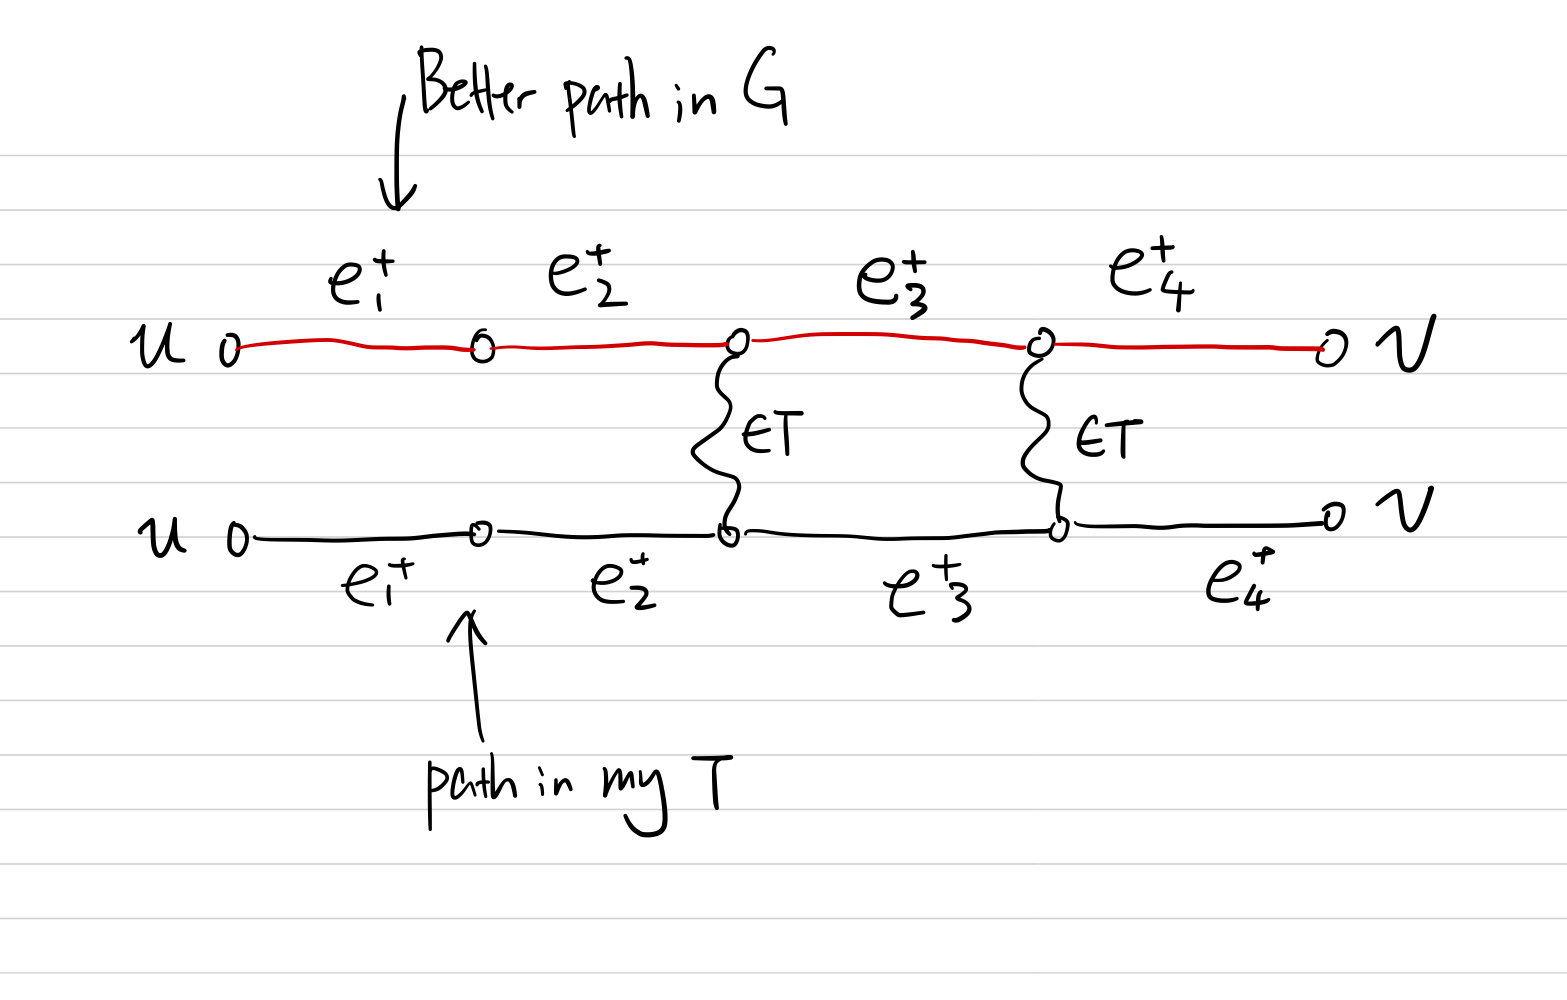
\includegraphics[width=10cm]{1.11.jpeg}    
    \end{center}
    Both $e_j^+$ and $e_i$ are in the cycle after the inclusion, all other edges already exists in the tree. Therefore: $T^+:= T\setminus \{e_i\}\cup \{e_j^+\}$ will improve $r_{T^+}(u, v)$ and $T^+$ is still a tree. Worth noting is that, the total weights of all the egdes in $T^+$ is larger: $l(T^+) > l(T)$ because $l(e_j^+) > l(e_i)$. And the path now has the best reliability giving us: $r_G(v_0, v_n) = r_{T^+}(v_0, v_n)$. 
    \\
    Repeat this process, redefining $T := T^+$ , do this for all paths in $G$ that has better reliability, then the weight of the tree $T^+$ improves monotonically. There is an upper bound to the total weight of the edges of the tree because $E$ is finite, therefore it has to be the case that there exists $T$ that has the best reliability, and when that happens, it includes all the best path in $G$, giving us $r_G(u, v) = r_T^+(u, v)\;\forall u, v \in V$. 


\end{document}